\documentclass[11pt]{article}

% ── ArXiv preprint style ──
\usepackage[margin=1in]{geometry}
\usepackage{natbib}

\usepackage[utf8]{inputenc}
\usepackage[T1]{fontenc}
\usepackage{hyperref}
\usepackage{url}
\usepackage{booktabs}
\usepackage{amsmath,amssymb}
\usepackage{graphicx}
\usepackage{xcolor}
\usepackage{multirow}
\usepackage{array}
\usepackage{enumitem}
\usepackage{algorithm}
\usepackage{algorithmic}
\usepackage{subcaption}
\usepackage{tablefootnote}
\usepackage{colortbl}
\usepackage{pifont}  % for \ding symbols
\usepackage{tikz}
\usetikzlibrary{arrows.meta,positioning,fit,backgrounds,calc,decorations.pathreplacing,patterns,shapes.geometric}
\usepackage{pgfplots}
\pgfplotsset{compat=1.18}
\usepgfplotslibrary{groupplots,fillbetween}
\usepackage{tcolorbox}
\tcbuselibrary{skins,breakable}

% ── Compact lists ──
\setlist{nosep,leftmargin=*}

% ── Color palette (NeurIPS-style, colorblind-friendly) ──
\definecolor{bestcolor}{HTML}{E8F5E9}
\definecolor{gaincolor}{HTML}{1B5E20}
\definecolor{cStandard}{HTML}{BF616A}   % muted red
\definecolor{cAOI}{HTML}{5E81AC}        % steel blue
\definecolor{cDelta}{HTML}{A3BE8C}      % sage green
\definecolor{cVisual}{HTML}{D08770}     % muted orange
\definecolor{cASR}{HTML}{B48EAD}        % muted purple
\definecolor{cNarr}{HTML}{88C0D0}       % light blue
\definecolor{cAccent}{HTML}{EBCB8B}     % warm yellow
\definecolor{cGray}{HTML}{4C566A}       % dark gray
\definecolor{cLightGray}{HTML}{D8DEE9}  % light gray

\title{\textbf{Agent-Computer Observation Interfaces\\Enable Dynamic Computer Use}}

\author{Anonymous Authors\\[2pt]
\small\url{https://anonymous.4open.science/r/aoi-anonymous}}

\begin{document}

\maketitle

% ════════════════════════════════════════════════════════════
\begin{abstract}
% ════════════════════════════════════════════════════════════
\textbf{The interface, not the model.}
Just as SWE-agent~\citep{sweagent} showed that the agent-computer \emph{action} interface is a critical and underexplored design axis for software-engineering agents, we show that the \emph{observation} interface is equally critical for computer-use (CU) agents---and that getting it right unlocks dynamic computer use from any existing CU model without retraining.
Current CU agents---closed-source and open-source alike---observe the world through periodic static screenshots taken every 3--5\,s and have no audio perception, leaving them unable to handle video playback, animations, transient UI events, meetings, notifications, or spoken instructions.
We introduce the \textbf{Agent Observation Interface (AOI)}, a lightweight, model-agnostic perception layer that decouples observation from action: observation runs continuous and adaptive in the background; action stays discrete.
The AOI has three gated components: (1)~inter-step keyframe capture, (2)~volume-gated audio scene understanding, and (3)~CU-model-generated visual narration that converts ephemeral keyframes into persistent text.
On static, silent content the gates produce nothing and behaviour is identical to the standard loop.

\textbf{Results.}
We introduce \textbf{DynaCU-Bench}, a benchmark of 100 dynamic browser tasks across 10 categories plus 50 static tasks for zero-overhead verification.
Six CU models---Claude Sonnet~4.6, GPT-5.4, Gemini~2.5~Flash, Grok-4, EvoCUA-32B, and Fara-7B---equipped with the AOI achieve absolute gains of +17 to +48 percentage points over their screenshot-only baselines (paired McNemar $p<10^{-3}$ for every model), with the strongest configuration reaching 82\% on Claude Sonnet~4.6 (Section~\ref{sec:variance} reports a 3-seed variance estimate for the headline number).
On a balanced 12-task audio-focused subset, AOI~full (12/12) substantially outperforms two production streaming baselines---the OpenAI Realtime API~\citep{openairealtime} (3/12) and Gemini~Live~\citep{geminilive} (0/12)---both adapted to drive the same browser environment, with an adapter-sanity check showing the failures are content-driven rather than infrastructural.

\textbf{Two surprises about the observation interface.}
A controlled ablation finds that \emph{selection doesn't matter, capture does}: four inter-step keyframe selection strategies (uniform, random, pixel-difference, and CLIP) are statistically indistinguishable (pairwise McNemar $p>0.5$, ${\sim}58\%$ each), a finding we replicate on the open-source Qwen3-VL-32B vision model.
ASR adds +6\,pp, and the largest single-component gain comes from \emph{persistent text memory}: a narration-discarded ablation isolates a significant $+8$\,pp contribution from retaining narration after keyframes are pruned ($p=0.039$ at $N{=}100$), plus a directional but underpowered $+10$\,pp from inference-time chain-of-thought during narration generation ($p=0.12$; reaching $p<0.05$ at this effect size would require $N{\sim}300$).
A direct \texttt{standard\_structured} control decomposes each cloud model's gain into a prompt-format component and a perception-only component; for the cloud models predating Gemini~3 both contribute positively (Claude: $+25$\,pp perception vs.\ $+19$\,pp prompt-format; Gemini~2.5~Flash: $+23$\,pp vs.\ $+25$\,pp).  For Gemini~3~Flash the headline residual collapses to $+9$\,pp ($p=0.18$, not significant at $N{=}100$).  A four-way decomposition (\texttt{standard}/\texttt{standard\_audio}/\texttt{aoi\_audio}/\texttt{aoi\_full}, 100 tasks each) explains this without invoking internalised perception: on Gemini~3 the AOI's three components have sign-separated effects---audio $+12$\,pp, structured scaffold $+9$\,pp (positive net, bi-directional per category), keyframes $\mathbf{-12}$\,pp.  Replacing the v10 keyframe-bearing bundle with \texttt{aoi\_audio} (audio$+$scaffold, no keyframes) reaches $57/100$, a $+21$\,pp recovery and $+12$\,pp above \texttt{aoi\_full}.  Implication: the keyframe component is the first AOI element we observe crossing from net-positive to net-negative across model generations, and component selection must therefore become per-model rather than a fixed bundle.
Together, these results sharpen the central design hypothesis: the observation interface is a separable, mechanism-driven design axis along which models converge unevenly \emph{and unevenly per component}.  The AOI's residual gain remains a diagnostic of where a model has slack---now with the additional caveat that the slack may live in any subset of (audio, structured presentation, keyframe imagery, action-policy compatibility), and the optimal AOI configuration is itself a per-model design choice.
\end{abstract}

% ════════════════════════════════════════════════════════════
\section{Introduction}
\label{sec:intro}
% ════════════════════════════════════════════════════════════

\textbf{The agent-computer observation interface as a design axis.}
SWE-agent~\citep{sweagent} made a contribution that, in retrospect, was not a new model: it was a careful design of the agent-computer \emph{action} interface---which commands a language model is given to act on a codebase, how their inputs and outputs are formatted, what feedback they return.
Their finding was sharp: small changes there dramatically affect what a fixed model can accomplish, and the action interface is therefore a separable, underexplored design axis.
We make the analogous argument for the \emph{observation} interface in computer-use (CU) agents.
Today, every CU agent we are aware of---closed-source~\citep{anthropic2024claude,openai2025cua,gemini25cu,surfer2} and open-source~\citep{uitars2,opencua,fara7b,coact}---ties observation to action: one screenshot per action step.
We argue this conflation is a design choice, not a necessity, and that decoupling observation (continuous, adaptive) from action (discrete) is the single change that unlocks dynamic computer use from any existing CU model with zero retraining.

\textbf{The current state.}
On OSWorld~\citep{osworld}, screenshot-based agents have moved from sub-10\% completion at the benchmark's introduction to over 50\% in 2025 (Surfer~2~\citep{surfer2}: 50.7\% under their cross-platform harness; UI-TARS-2~\citep{uitars2}: 47.5\%), closing most of the gap to the 72.4\% human baseline.
These agents can operate real desktops: filling forms, navigating websites, editing documents, and using professional software.

\textbf{The blind spot.}
All these agents share a fundamental architectural limitation: they observe the world through \emph{discrete static screenshots} taken every 3--5 seconds, and they are entirely deaf.
Between screenshots, the agent is completely blind.
This makes current CU agents incapable of understanding video content playing on screen, catching transient UI events that appear and auto-dismiss between observations, hearing meeting speech or notification sounds, or perceiving animations that convey information.
A recent comprehensive survey of CU agents~\citep{cusurvey} catalogs many open challenges but does not identify the observation modality as a gap.
Quantitative evidence of this limitation is mounting: GUI-World~\citep{guiworld} shows video LLMs fail on all temporal GUI tasks; VideoWebArena~\citep{videowebarena} reports that long-context models perform \emph{worse} with video than without; VideoGameBench~\citep{videogamebench} finds even paused-game evaluation yields only 1.6\% completion; and CUA-Suite~\citep{cuasuite} demonstrates the richness of temporal dynamics that screenshot-based agents entirely miss across 55 hours of desktop recordings.

\textbf{Why existing approaches fall short.}
Retraining CU models on video data is expensive, model-specific, and undemonstrated at scale.
Using video-native models (Gemini) amounts to brute-force frame sampling that wastes tokens on redundant static frames.
Native real-time multimodal models (Gemini Live~\citep{geminilive}, OpenAI Realtime~\citep{openairealtime}) work but lock users into a single provider, offer no selective perception, and require API migration; we evaluate them in Section~\ref{sec:streaming}.
General control frameworks like Cradle~\citep{cradle} include pixel-level frame differencing but lack audio perception, visual narration, and the structured observation record.

\textbf{Our approach.}
The bridge is the \textbf{Agent Observation Interface (AOI)}, a lightweight perception layer that converts continuous screen and audio streams into the sparse images and text that existing CU models already accept.
The AOI sits between the environment and any image-based CU model; on static, silent content its gates produce nothing and behaviour reverts to the standard loop; on dynamic content it produces extra keyframes, audio transcripts, and CU-model-generated narration that persists as text after the source images are pruned.

\textbf{Contributions.}
\begin{enumerate}
  \item We identify the \textbf{observation interface} as a critical but overlooked design axis in CU agents, complementary to the action interface studied by SWE-agent, and articulate \emph{decoupling observation from action} as the operative design principle.
  \item We introduce the \textbf{AOI}, a model-agnostic perception layer with three gated components (inter-step keyframe capture, volume-gated audio scene understanding, and CU-model-generated visual narration that persists as text).
  \item We introduce \textbf{DynaCU-Bench} (100 dynamic tasks) and a \textbf{Static-50} no-degradation baseline.  (A cross-engine ASR check using \texttt{espeak} and real asciinema cast files is reported in Appendix~\ref{app:realcontent} as a no-degradation pilot, not a perception comparison.)
  \item We demonstrate that six CU models equipped with the AOI and \textbf{zero retraining} achieve absolute gains of +17 to +48 percentage points on dynamic tasks (paired McNemar $p<10^{-3}$ for every model).
  \item We show via a controlled \emph{narration-discarded} ablation that the visual-narration component's $+18$\,pp gain decomposes into a significant $+8$\,pp from \emph{persistent text memory} of past visual observations ($p=0.039$) plus a directional, underpowered $+10$\,pp from inference-time chain-of-thought during narration generation ($p=0.12$ at $N{=}100$).
  \item We rule out two important confounds: a direct \texttt{standard\_structured} run on DynaCU-Bench separates the AOI's structured-prompt effect from its perception effect (Section~\ref{sec:static}), and an open-source replication on Qwen3-VL-32B confirms the selection-method convergence is mechanism-driven, not Claude-specific (Section~\ref{sec:ablation}).
  \item We benchmark against monolithic streaming baselines (Gemini Live~\citep{geminilive}, OpenAI Realtime~\citep{openairealtime}) with a separate adapter sanity check (Section~\ref{sec:streaming}, Appendix~\ref{app:streaming_sanity}).
\end{enumerate}

% ════════════════════════════════════════════════════════════
\section{Background: The CU Agent Loop}
\label{sec:background}
% ════════════════════════════════════════════════════════════

All current CU agents follow the same observe--reason--act loop:
\begin{equation}
  \texttt{repeat:}\quad s_t \leftarrow \text{Screenshot}(),\quad a_t \leftarrow \text{CU\_Model}(s_t, \tau),\quad \text{Execute}(a_t),\quad \text{Wait}(\delta)
  \label{eq:culoop}
\end{equation}
where $\tau$ is the trajectory history and $\delta$ is a post-action buffer (typically 500\,ms).
The interval between observations is determined by model inference time + action execution + buffer, typically 3--5 seconds total.
Everything that occurs between screenshots---visual changes, audio events, transient UI elements---is invisible to the agent.

Some models support multi-image input through screenshot history (UI-TARS: up to 5 images, Claude CU: ${\sim}10$), but all images are post-action screenshots from prior steps.
None captures what happens \emph{between} steps.

Four categories of content are systematically missed:
(i)~\emph{transient UI events}---toast notifications and dialogs that appear and vanish within one observation interval;
(ii)~\emph{continuous visual media}---video playback, animated tutorials, transitioning slides;
(iii)~\emph{audio events}---meeting speech, notification sounds, error alerts;
(iv)~\emph{periodic visual noise}---loading spinners and blinking cursors that should be \emph{ignored} but trigger false positives in naive frame differencing.

% ════════════════════════════════════════════════════════════
\section{System Design}
\label{sec:design}
% ════════════════════════════════════════════════════════════

The AOI sits between the environment and any existing CU model.
It observes the entire interval between agent steps and provides the CU model with additional keyframes, audio descriptions, and accumulated text context---all in the standard image + text format that every CU model already accepts.
For static, silent tasks, the AOI produces nothing and behavior is identical to the standard loop.
For dynamic tasks, the CU model receives strictly more information.
No retraining is needed.

\subsection{Architecture Overview}

The AOI has three components, each preceded by a fast gate (sub-millisecond) that short-circuits processing when there is nothing to perceive.
For a frame that passes the gates, the additional cost is dominated by CLIP-ViT-B/16 (${\sim}7$\,ms on GPU) for visual frames and Whisper large-v3 (variable, on demand) for audio segments; for the static, silent frames that dominate most workloads the per-frame cost is the sub-millisecond gate alone.

\begin{enumerate}[label=(\arabic*)]
  \item \textbf{Inter-step keyframe capture}: continuous screen sampling at ${\sim}3$\,Hz with gating to suppress redundant frames. Produces 0--5 keyframe images per step.
  \item \textbf{Volume-gated audio observer}: RMS energy gate followed by ASR (Whisper large-v3). Produces a text transcription per step, only when audio is present.
  \item \textbf{Visual narration context}: the CU model itself generates a brief text description of new visual information as a side-output of each inference call. These narrations accumulate in the trajectory and persist after keyframe images are pruned from context.
\end{enumerate}

\begin{figure*}[t]
\centering
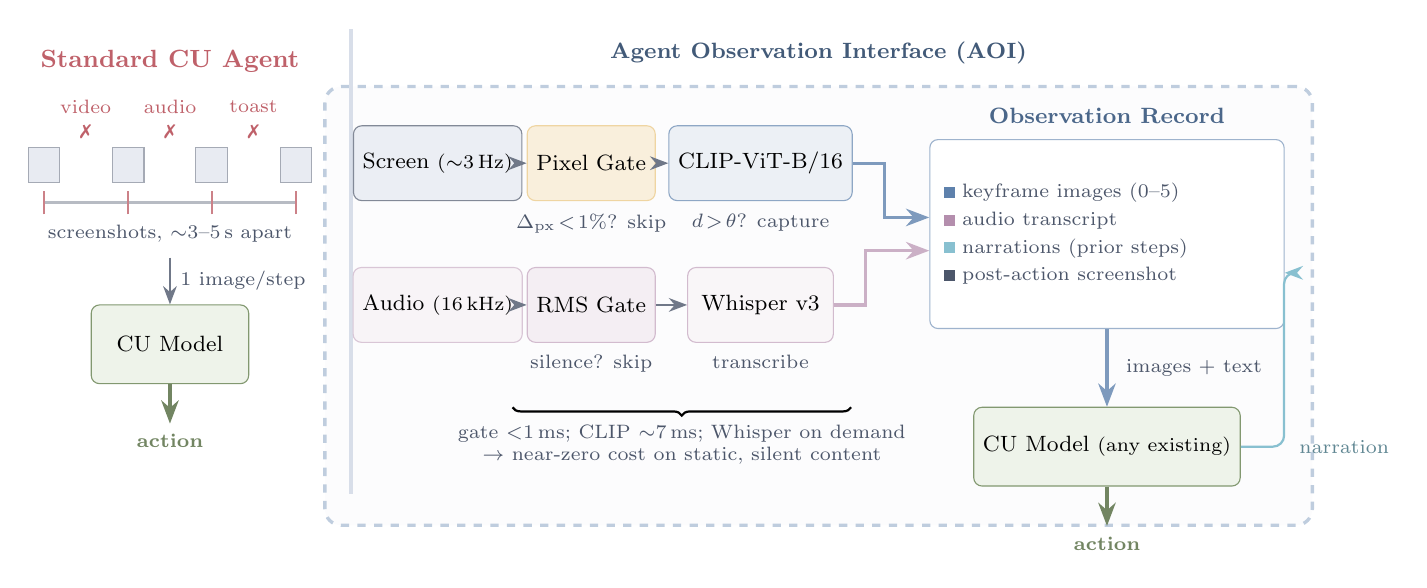
\begin{tikzpicture}[
    >=Stealth,
    box/.style={draw, rounded corners=3pt, minimum height=0.95cm, align=center, font=\footnotesize},
    env/.style={box, fill=cLightGray!50, draw=cGray!70, minimum width=1.6cm},
    gate/.style={box, fill=cAccent!30, draw=cAccent!80, minimum width=1.55cm},
    proc/.style={box, fill=cAOI!12, draw=cAOI!70, minimum width=1.85cm},
    obs/.style={box, fill=white, draw=cAOI!60, minimum width=4.5cm, minimum height=2.4cm},
    mdl/.style={box, fill=cDelta!18, draw=cDelta!80!black, minimum width=2.6cm, minimum height=1cm},
    arr/.style={->, thick, cGray!80},
    harr/.style={->, very thick, cAOI!80},
    lbl/.style={font=\scriptsize, text=cGray},
  ]
  % ── Left: Standard CU Agent ──
  \node[font=\small\bfseries, text=cStandard] at (1.6, 4.2) {Standard CU Agent};

  % Timeline with screenshots
  \draw[thick, cGray!40] (0, 2.4) -- (3.2, 2.4);
  \foreach \x in {0, 1.07, 2.13, 3.2} {
    \draw[thick, cStandard!80] (\x, 2.25) -- (\x, 2.55);
    \draw[cGray!50, fill=cLightGray!60] (\x-0.2, 2.65) rectangle (\x+0.2, 3.1);
  }
  \node[font=\scriptsize, text=cGray] at (1.6, 2.0) {screenshots, $\sim$3--5\,s apart};

  % Blind gaps with X marks
  \foreach \x/\t in {0.53/video, 1.6/audio, 2.66/toast} {
    \node[font=\scriptsize, text=cStandard] at (\x, 3.30) {\ding{55}};
    \node[font=\scriptsize, text=cStandard] at (\x, 3.62) {\t};
  }

  % Model
  \node[mdl, minimum width=2.0cm] (sm) at (1.6, 0.6) {CU Model};
  \draw[arr] (1.6, 1.7) -- (sm.north) node[midway, right, lbl] {1 image/step};
  \draw[arr, cDelta!70!black, very thick] (sm.south) -- ++(0,-0.5)
    node[below, font=\scriptsize\bfseries, text=cDelta!70!black] {action};

  % ── Divider ──
  \draw[very thick, cLightGray] (3.9, -1.3) -- (3.9, 4.6);

  % ── Right: AOI Pipeline ──

  % Input streams
  \node[env] (scr) at (5.0, 2.9) {Screen {\scriptsize($\sim$3\,Hz)}};
  \node[env, fill=cASR!10, draw=cASR!50] (aud) at (5.0, 1.1) {Audio {\scriptsize(16\,kHz)}};

  % Gates
  \node[gate] (pg) at (6.95, 2.9) {Pixel Gate};
  \node[gate, fill=cASR!15, draw=cASR!60] (rg) at (6.95, 1.1) {RMS Gate};

  \draw[arr] (scr) -- (pg);
  \draw[arr] (aud) -- (rg);

  % Gate sublabels (between rows; tight to box)
  \node[font=\scriptsize, text=cGray, anchor=north, yshift=-1pt] at (pg.south) {$\Delta_\text{px}\!<\!1\%$? skip};
  \node[font=\scriptsize, text=cGray, anchor=north, yshift=-1pt] at (rg.south) {silence? skip};

  % Processors
  \node[proc] (clip) at (9.1, 2.9) {CLIP-ViT-B/16};
  \node[proc, fill=cASR!8, draw=cASR!60] (wh) at (9.1, 1.1) {Whisper v3};

  \draw[arr] (pg) -- (clip);
  \draw[arr] (rg) -- (wh);

  % Processor sublabels (between rows; tight to box)
  \node[font=\scriptsize, text=cGray, anchor=north, yshift=-1pt] at (clip.south) {$d\!>\!\theta$? capture};
  \node[font=\scriptsize, text=cGray, anchor=north, yshift=-1pt] at (wh.south) {transcribe};

  % Observation Record (further right; title above box, below AOI banner)
  \node[obs] (orec) at (13.5, 2.0) {};
  \node[font=\footnotesize\bfseries, text=cAOI!80!black, anchor=south, yshift=2pt] at (orec.north) {Observation Record};
  \node[font=\scriptsize, text=cGray, align=left, anchor=west] at (11.30, 2.00) {%
    \textcolor{cAOI}{\rule{4pt}{4pt}} keyframe images (0--5)\\[2pt]
    \textcolor{cASR}{\rule{4pt}{4pt}} audio transcript\\[2pt]
    \textcolor{cNarr}{\rule{4pt}{4pt}} narrations (prior steps)\\[2pt]
    \textcolor{cGray}{\rule{4pt}{4pt}} post-action screenshot};

  \draw[harr] (clip.east) -- ++(0.4,0) |- ([yshift=6pt]orec.west);
  \draw[harr, cASR!70] (wh.east) -- ++(0.4,0) |- ([yshift=-6pt]orec.west);

  % CU Model (placed below the Observation Record)
  \node[mdl] (cm) at (13.5, -0.7) {CU Model {\scriptsize(any existing)}};
  \draw[harr, very thick] (orec.south) -- (cm.north)
    node[midway, right=3pt, lbl] {images + text};

  % Narration feedback loop (routed around the right side)
  \draw[harr, cNarr, thick, rounded corners=4pt]
    (cm.east) -- ++(0.55,0) coordinate (narrcorner) |- ([yshift=-14pt]orec.east);
  \node[font=\scriptsize, text=cNarr!70!black, anchor=west, xshift=2pt] at (narrcorner) {narration};

  % Action output
  \draw[arr, very thick, cDelta!70!black] (cm.south) -- ++(0, -0.5)
    node[below, font=\scriptsize\bfseries, text=cDelta!70!black] {action};

  % Brace annotation for gates (kept to gate+processor band, two-line label)
  \draw[thick, decorate, decoration={brace, amplitude=3pt, mirror}]
    (5.95, -0.20) -- (10.25, -0.20);
  \node[font=\scriptsize, text=cGray, align=center, anchor=north] at (8.1, -0.30) {%
    gate $<$1\,ms; CLIP $\sim$7\,ms; Whisper on demand\\
    $\to$ near-zero cost on static, silent content};

  % ── AOI bounding box ──
  \begin{scope}[on background layer]
    \node[draw=cAOI!40, line width=1.2pt, dashed, rounded corners=6pt, fill=cAOI!2,
          inner xsep=10pt, inner ysep=14pt,
          fit=(scr)(aud)(pg)(rg)(clip)(wh)(orec)(cm),
          label={[font=\footnotesize\bfseries, text=cAOI!70!black, anchor=south, yshift=4pt]above:Agent Observation Interface (AOI)}] {};
  \end{scope}

\end{tikzpicture}
\caption{\textbf{Standard CU agents vs.\ AOI-equipped agents.}
\emph{Left:} Current agents observe through periodic screenshots (${\sim}$3--5\,s apart) and are blind and deaf between observations---missing video, audio, and transient UI events (\ding{55}).
\emph{Right:} The AOI continuously monitors screen and audio streams through fast gates ($<$1\,ms) that skip processing for static, silent content.
When gates fire, keyframe extraction (shown here with optional CLIP filtering; see Section~\ref{sec:ablation}) and Whisper ASR produce images and text for the observation record.
Visual narrations feed back as persistent text memory.
The AOI wraps any existing CU model with zero retraining.}
\label{fig:architecture}
\end{figure*}

\subsection{Inter-Step Keyframe Capture}
\label{sec:keyframes}

Between agent steps, the screen may change (a video plays, a dialog appears, a slide transitions) or stay static.
The AOI continuously samples the screen at ${\sim}3$\,Hz and selects a subset of frames to include as keyframe images in the observation record (up to 5 per step).
Multiple selection strategies are possible---uniform fixed-rate sampling, pixel-level differencing, random sampling, or semantic filtering via CLIP embeddings~\citep{clip}.
We evaluate all four in Section~\ref{sec:ablation} and find that all converge to similar accuracy, so the default implementation uses simple pixel-change gating: if fewer than 1\% of pixels changed since the last captured frame, the sample is skipped (cost: ${<}1$\,ms on CPU).
For static screens, no keyframes are produced and the component has zero overhead.
Algorithm~\ref{alg:keyframe} formalises the two-stage CLIP variant; the default selector drops the CLIP stage (lines~5--10) and uses only Stage~1.

\begin{algorithm}[t]
\caption{Two-stage adaptive keyframe extraction (CLIP variant).
This algorithm is shown for completeness; the selection-method ablation in
Section~\ref{sec:ablation} finds it statistically indistinguishable from
the simpler pixel-only gate (Stage~1) and uniform / random sampling, so the
default selector in every main result is Stage~1 alone.}
\label{alg:keyframe}
\begin{algorithmic}[1]
\REQUIRE Screen sample $x_t$, anchor embedding $e_\text{anchor}$, pixel threshold $\alpha$, CLIP threshold $\theta$
\STATE $\Delta_\text{px} \leftarrow \text{PixelChangeRatio}(x_t, x_\text{prev})$
\IF{$\Delta_\text{px} < \alpha$}
  \RETURN \textsc{Skip} \COMMENT{Stage 1: no pixel change}
\ENDIF
\STATE $e_t \leftarrow \text{CLIP}(x_t)$
\STATE $d \leftarrow 1 - \cos(e_t, e_\text{anchor})$
\IF{$d > \theta$}
  \STATE $e_\text{anchor} \leftarrow e_t$ \COMMENT{Re-anchor}
  \RETURN \textsc{CaptureKeyframe}($x_t$, $t$)
\ENDIF
\RETURN \textsc{Skip} \COMMENT{Stage 2: below semantic threshold}
\end{algorithmic}
\end{algorithm}

\subsection{Volume-Gated Audio Observation}
\label{sec:audio}

Current CU agents have zero audio perception.
They cannot hear meeting speech, notification sounds, or error alerts.
Pure ASR models (Whisper) transcribe speech but produce nothing for non-speech audio events.

\textbf{Volume gate.}
In most computer use---file editing, form filling, silent web browsing---there is no audio.
Computing RMS energy of the audio buffer is sub-millisecond.
If below the silence threshold, the audio model call is skipped entirely.
Cost: ${\sim}0$\,ms for the majority of steps.

When audio is present, we use Whisper large-v3~\citep{whisper} for speech transcription, operating on 16\,kHz mono audio captured from the system audio output via PulseAudio virtual devices.
The audio buffer spans the full inter-step interval including the post-action buffer, capturing action feedback sounds (click confirmations, error beeps).

\textbf{Overlapping windows.}
Agent step boundaries are determined by model inference latency, not by speech content.
A typical 3.5-second audio chunk captures ${\sim}8$--9 words at normal speaking rate, almost always falling mid-sentence.
To resolve boundary artifacts, the audio buffer includes ${\sim}3.5$ seconds of overlap from the previous interval, providing acoustic continuity across step boundaries.

\subsection{Visual Narration for Long-Term Context}
\label{sec:narration}

CU models retain only the most recent images in context.
Keyframes from earlier steps are pruned.
For tasks spanning many steps, the agent loses all visual memory of earlier content.
Audio transcriptions persist naturally as text in the trajectory, but visual observations have no analogous persistence.

At each step, the CU model outputs both an action and a brief visual narration---a text description of what is visually new in the current keyframes.
This narration is generated in the same inference call that produces the action (zero additional compute) and persists indefinitely in the trajectory, even after the corresponding images are pruned.
Following the caption-then-reason principle of LLoVi~\citep{llovi}, narrations are generated by the CU model itself (no separate captioner) and are task-relevant rather than generic.

\subsection{Observation Record}
\label{sec:obsrecord}

At each step, the CU model receives a structured document combining text context from recent prior steps (audio transcriptions, visual narrations, actions taken) and raw observations from the current interval (new audio transcription, any captured keyframe images, and the post-action screenshot).
For static, silent tasks, this document contains only the post-action screenshot---identical to the standard loop.
Figure~\ref{fig:obsrecord} shows a concrete example.

\begin{figure}[t]
\centering
\begin{tcolorbox}[
  colback=gray!3, colframe=black!40,
  title={\small\bfseries Observation Record --- Step $N$ (Meeting Task B-E1)},
  fonttitle=\small, coltitle=white, colbacktitle=black!60,
  width=0.95\textwidth, boxrule=0.4pt,
]
\ttfamily\scriptsize
\textcolor{blue!70!black}{\# CONTEXT --- text from prior steps (no images)}\\[2pt]
\textbf{Step N-1} (t $\approx$ 18.5--22.0\,s):\\
\quad AUDIO: ``Here's the team. As you can see we\\
\qquad have strong cross-functional coverage.''\\
\quad VISUAL: ``Meeting slide shows Project Team\\
\qquad with 6 members listed in a grid.''\\
\quad ACTION: wait()\\[4pt]
%
\textcolor{blue!70!black}{\# NEW --- current interval observations}\\[2pt]
\textbf{Step N} (t $\approx$ 22.0--25.5\,s):\\
\quad AUDIO: ``And I want to mention, we've moved\\
\qquad the launch date to April 28th.\\
\qquad Please update your calendars.''\\[2pt]
\quad \textcolor{gray}{[IMAGE: post-action screenshot]}\\[4pt]
%
\textcolor{blue!70!black}{\# TASK}\\
\quad Read the meeting slides and listen to the\\
\quad discussion. What is the new launch date?\\
\quad Enter it in the Launch Date field.
\end{tcolorbox}
\caption{Example observation record sent to the CU model at step $N$ of a meeting task.
The \textbf{context} section provides text from prior steps (audio transcriptions and visual narrations persist after images are pruned).
The \textbf{new} section contains the current audio transcription and the post-action screenshot (image).
In this case, no keyframes were captured (the slide did not change), so only the screenshot is included as an image.
The task instruction is appended at the end.}
\label{fig:obsrecord}
\end{figure}

% ════════════════════════════════════════════════════════════
\section{Implementation}
\label{sec:implementation}
% ════════════════════════════════════════════════════════════

The AOI is implemented in Python (${\sim}2{,}600$ lines) as a modular layer that wraps any CU model.
Screen capture uses a headless browser (Playwright) at ${\sim}3$\,Hz.
Audio capture and injection use PulseAudio virtual devices (virtual speaker and monitor source) at 16\,kHz mono.
CLIP-ViT-B/16 runs on GPU (${\sim}150$\,MB VRAM).
Whisper large-v3 runs as a separate HTTP service on CPU to avoid GPU contention with the CU model.
Audio synthesis for benchmark tasks uses the Web Speech API (\texttt{speechSynthesis}).

CU models are accessed through their native APIs.
Cloud models (Claude Sonnet~4.6, GPT-5.4, Gemini~2.5 Flash) use HTTP APIs.
Local models (EvoCUA-32B, Fara-7B) are served via vLLM with 4-bit quantization on a single NVIDIA RTX PRO 6000 (96\,GB VRAM).

% ════════════════════════════════════════════════════════════
\section{DynaCU-Bench}
\label{sec:benchmark}
% ════════════════════════════════════════════════════════════

\subsection{Design Principles}

Existing CU benchmarks~\citep{osworld,webarena,webvoyager} consist almost entirely of tasks solvable from static screenshots.
We introduce \textbf{DynaCU-Bench}, a benchmark of 100 browser-based tasks that specifically require dynamic visual and/or audio perception---tasks that are unsolvable from static screenshots alone.

Design principles:
(i)~tasks must \emph{require} temporal visual or audio perception;
(ii)~tasks represent realistic computer-use scenarios, not artificial constructs;
(iii)~tasks execute in a reproducible headless browser environment;
(iv)~tasks cover all four dynamic content categories from Section~\ref{sec:background};
(v)~tasks include difficulty stratification (3 easy, 4 medium, 3 hard per category).

\subsection{Task Categories}

DynaCU-Bench spans 10 categories across three capability axes: audio perception~(A), visual-temporal perception~(V), and real-time interaction~(I). Each category has 10 tasks.

\begin{table}[t]
\centering
\caption{DynaCU-Bench task categories.
A = audio perception, V = visual-temporal perception, I = real-time interaction.
Each category contains 3 easy, 4 medium, and 3 hard tasks.}
\label{tab:categories}
\small
\begin{tabular}{@{}llcp{6.8cm}@{}}
\toprule
\textbf{Cat.} & \textbf{Domain} & \textbf{Axes} & \textbf{Description} \\
\midrule
A & Podcast comprehension & A & Listen to audio narration, extract facts or answer questions \\
B & Meeting participation & A+V+I & Follow meeting with slides and speech, take notes or act \\
C & Video/screencast & V & Watch terminal recordings or IDE demos with auto-advancing frames \\
D & Carousel/animation & V & Perceive CSS transitions, rotating content, product carousels \\
E & Live dashboard & V & Monitor real-time updating dashboards with \texttt{setInterval} changes \\
F & Transient UI events & V & Respond to toast notifications, auto-dismissing banners \\
G & Phone/voice call & A+I & Listen to \texttt{speechSynthesis} calls and respond \\
H & Interview/voice & A+I & Answer questions via \texttt{SpeechRecognition}, complete interviews \\
I & Collaborative editing & V+I & Handle remote changes in collaborative document editors \\
J & Browser games & V+I & Play interactive games requiring temporal attention \\
\bottomrule
\end{tabular}
\end{table}

\subsection{Evaluation Protocol}

Each task executes in a headless Chromium browser (Playwright) with PulseAudio virtual devices for audio I/O.
Audio content is delivered via the Web Speech API (\texttt{speechSynthesis}) with edge-TTS for high-quality voices.
Agent audio input is injected into a virtual microphone via \texttt{pacat}.

Three evaluation modes are used:
\emph{DOM-based} (93 tasks): a deterministic JavaScript function \texttt{getTaskResult()} returns the expected value;
\emph{LLM-judged} (1 task): a judge model scores the agent's response against a rubric;
\emph{Hybrid} (6 tasks): DOM gate (did the agent act?) combined with LLM quality assessment.
All tasks allow a maximum of 15 agent steps.

% ════════════════════════════════════════════════════════════
\section{Evaluation}
\label{sec:eval}
% ════════════════════════════════════════════════════════════

\subsection{Setup}

\textbf{CU models.}
We evaluate six models spanning the capability and scale spectrum:
(i)~Claude Sonnet~4.6 \citep{anthropic2024claude} (closed-source);
(ii)~GPT-5.4 \citep{openai2026gpt54} (closed-source; the latest GPT-5 series tool-calling-capable vision model exposed by OpenAI's chat-completions API at evaluation time);
(iii)~Gemini~2.5~Flash \citep{gemini25cu} (closed-source);
(iv)~Grok-4 \citep{xai2026grok4} (closed-source, xAI; reported in Section~\ref{sec:grok} with attention to the inference-latency confound);
(v)~EvoCUA-32B \citep{evocua} (open-source, 32B; weights and inference recipe released through Meituan's GitHub);
(vi)~Fara-7B \citep{fara7b} (open-source, 7B).
We use each model's vendor-recommended decoding settings (temperature, top-$p$) unchanged.
We do not rely on any vendor-reported OSWorld score for any claim in this paper; we report only the numbers measured under our own DynaCU-Bench harness.

\textbf{Observation configurations.}
We compare 8 observation modes:
\begin{enumerate}[label=(\arabic*)]
  \item \textbf{Standard}: one screenshot per step, no audio (current paradigm baseline).
  \item \textbf{Uniform 1\,FPS}: capture at fixed 1\,FPS, feed recent $N$ frames.
  \item \textbf{Uniform 3\,FPS}: capture at fixed 3\,FPS, feed recent $N$ frames.
  \item \textbf{Pixel-diff}: capture when pixel change ratio exceeds threshold, no CLIP filtering.
  \item \textbf{Random keyframes}: randomly sample the same number of frames as our method.
  \item \textbf{AOI (visual only)}: adaptive keyframes (CLIP-based), no audio.
  \item \textbf{AOI (visual + ASR)}: adaptive keyframes + Whisper speech transcription.
  \item \textbf{AOI (full)}: adaptive keyframes + Whisper ASR + visual narration.
\end{enumerate}
Ablation configurations (2)--(7) are evaluated with Claude Sonnet~4.6; the full AOI and standard baseline are evaluated with all five models.

\subsection{Main Results}

\begin{table}[t]
\centering
\caption{DynaCU-Bench results: task success rate (\%) on the 100 dynamic tasks.
Brackets show 95\% Wilson confidence intervals.
\textbf{Bold} indicates the best result per model. $\Delta$ is the absolute gain over the standard baseline; $p$-values are paired McNemar's exact mid-$p$ tests.
All ablation modes are tested on Claude Sonnet~4.6.
``Claude 4.6'' abbreviates Claude Sonnet~4.6 throughout.
Grok-4 is the slowest model at inference (${\sim}80$--180\,s/call), which holds its absolute scores down even when AOI unblocks perception; see Section~\ref{sec:grok}.}
\label{tab:main}
\small
\setlength{\tabcolsep}{3.0pt}
\begin{tabular}{@{}lcccccc@{}}
\toprule
\textbf{Configuration} & \textbf{Claude 4.6} & \textbf{GPT-5.4} & \textbf{Gemini 2.5} & \textbf{Grok-4} & \textbf{EvoCUA-32B} & \textbf{Fara-7B} \\
\midrule
Standard (screenshot) & 38 \scriptsize[29.1, 47.8] & 37 \scriptsize[28.2, 46.8] & 21 \scriptsize[14.2, 30.0] & 4 \scriptsize[1.6, 9.8] & 18 \scriptsize[11.7, 26.7] & 17 \scriptsize[10.9, 25.5] \\
\midrule
Uniform 1\,FPS & 58 \scriptsize[48.2, 67.2] & --- & --- & --- & --- & --- \\
Uniform 3\,FPS & 56 \scriptsize[46.2, 65.3] & --- & --- & --- & --- & --- \\
Pixel-diff only & 58 \scriptsize[48.2, 67.2] & --- & --- & --- & --- & --- \\
Random keyframes & 56 \scriptsize[46.2, 65.3] & --- & --- & --- & --- & --- \\
\midrule
AOI (visual only) & 58 \scriptsize[48.2, 67.2] & --- & --- & --- & --- & --- \\
AOI (visual + ASR) & 64 \scriptsize[54.2, 72.7] & --- & --- & --- & --- & --- \\
\rowcolor{bestcolor}
\textbf{AOI (full)} & \textbf{82} \scriptsize[73.3, 88.3] & \textbf{57} \scriptsize[47.2, 66.3] & \textbf{69} \scriptsize[59.4, 77.2] & \textbf{25} \scriptsize[17.5, 34.4] & \textbf{55} \scriptsize[45.2, 64.4] & \textbf{34} \scriptsize[25.5, 43.7] \\
\midrule
\textcolor{gaincolor}{$\Delta$ (full $-$ std)} & \textcolor{gaincolor}{+44} & \textcolor{gaincolor}{+20} & \textcolor{gaincolor}{+48} & \textcolor{gaincolor}{+21} & \textcolor{gaincolor}{+37} & \textcolor{gaincolor}{+17} \\
\textit{p (McNemar)} & \scriptsize $1.3{\times}10^{-10}$ & \scriptsize $8.8{\times}10^{-5}$ & \scriptsize $2.9{\times}10^{-12}$ & \scriptsize $3.0{\times}10^{-6}$ & \scriptsize $3.0{\times}10^{-9}$ & \scriptsize $4.9{\times}10^{-4}$ \\
\bottomrule
\end{tabular}
\end{table}

\begin{figure}[t]
\centering
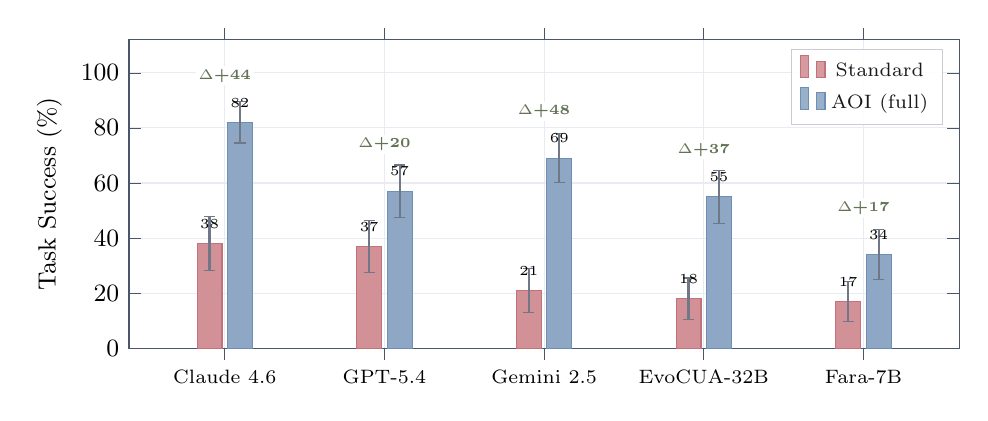
\begin{tikzpicture}
\begin{axis}[
    width=\columnwidth,
    height=5.5cm,
    ybar,
    bar width=9pt,
    ymin=0, ymax=112,
    ylabel={Task Success (\%)},
    ylabel style={font=\small},
    symbolic x coords={Claude 4.6, GPT-5.4, Gemini 2.5, EvoCUA-32B, Fara-7B},
    xtick=data,
    xticklabel style={font=\scriptsize},
    ytick={0,20,40,60,80,100},
    yticklabel style={font=\small},
    legend style={at={(0.98,0.97)}, anchor=north east, font=\scriptsize,
                  draw=cGray!30, fill=white, fill opacity=0.9},
    grid=major,
    major grid style={cLightGray!60},
    axis line style={cGray},
    tick style={cGray},
    enlarge x limits=0.15,
    nodes near coords,
    nodes near coords style={font=\tiny\bfseries, /pgf/number format/fixed},
    every node near coord/.append style={above=2pt},
    clip=false,
]
% Standard bars with 95% Wilson CIs
\addplot[fill=cStandard!70, draw=cStandard!90,
         error bars/.cd, y dir=both, y explicit, error bar style={cGray!80, thick}]
    coordinates {
      (Claude 4.6,    38) +- (0, 9.78)
      (GPT-5.4,       37) +- (0, 9.45)
      (Gemini 2.5,    21) +- (0, 7.92)
      (EvoCUA-32B,    18) +- (0, 7.50)
      (Fara-7B,       17) +- (0, 7.31)
    };
\addplot[fill=cAOI!70, draw=cAOI!90,
         error bars/.cd, y dir=both, y explicit, error bar style={cGray!80, thick}]
    coordinates {
      (Claude 4.6,    82) +- (0, 7.49)
      (GPT-5.4,       57) +- (0, 9.55)
      (Gemini 2.5,    69) +- (0, 8.92)
      (EvoCUA-32B,    55) +- (0, 9.61)
      (Fara-7B,       34) +- (0, 9.09)
    };
\legend{Standard, AOI (full)}

% Delta annotations — positioned well above AOI nodes near coords labels
\node[font=\tiny\bfseries, text=cDelta!60!black, fill=white, inner sep=1pt, rounded corners=1pt]
    at (axis cs:Claude 4.6, 99) {$\Delta$+44};
\node[font=\tiny\bfseries, text=cDelta!60!black, fill=white, inner sep=1pt, rounded corners=1pt]
    at (axis cs:GPT-5.4, 74) {$\Delta$+20};
\node[font=\tiny\bfseries, text=cDelta!60!black, fill=white, inner sep=1pt, rounded corners=1pt]
    at (axis cs:Gemini 2.5, 86) {$\Delta$+48};
\node[font=\tiny\bfseries, text=cDelta!60!black, fill=white, inner sep=1pt, rounded corners=1pt]
    at (axis cs:EvoCUA-32B, 72) {$\Delta$+37};
\node[font=\tiny\bfseries, text=cDelta!60!black, fill=white, inner sep=1pt, rounded corners=1pt]
    at (axis cs:Fara-7B, 51) {$\Delta$+17};

\end{axis}
\end{tikzpicture}
\caption{\textbf{Main results on DynaCU-Bench (100 tasks).}
The AOI produces large gains across all five CU models without any retraining.
Green numbers show absolute improvement in percentage points.
Gemini~2.5 Flash shows the largest absolute gain (+48\,pp) and relative gain ($3.3\times$), while Claude achieves the highest absolute score (82\%).
Error bars are approximate 95\% intervals using a symmetric Gaussian span; exact (asymmetric) Wilson intervals are tabulated in Table~\ref{tab:main} and used for all reported $p$-values.}
\label{fig:mainresults}
\end{figure}

Table~\ref{tab:main} and Figure~\ref{fig:mainresults} present the main results.
The AOI produces large, consistent gains across all five models, all highly significant by paired McNemar's exact test ($p<10^{-3}$ for every model; $p<10^{-9}$ for Claude, Gemini, and EvoCUA).
\emph{Note on statistical power:} Each configuration is evaluated once on 100 binary-outcome tasks (no repeated trials).
We use paired McNemar's exact mid-$p$ tests on the discordant tasks to assess significance and report 95\% Wilson confidence intervals on the marginal success rates.
Pairwise differences between selection methods (e.g., 56\% vs.\ 58\%) are not significant ($p>0.5$ for every pair, see Table~\ref{tab:ablation}); the large between-tier gaps are.

\textbf{Claude Sonnet~4.6} improves from 38\% to 82\% (+44 pp) with the full AOI.
This is the strongest absolute result.
The ablation modes reveal that all inter-step visual capture methods converge to 56--58\% (a +18--20\,pp gain from additional frames alone, regardless of selection method), adding ASR reaches 64\%, and visual narration provides the largest single-component gain, reaching 82\%.
Section~\ref{sec:narration_discard} decomposes this $+18$\,pp gap into a significant $+8$\,pp persistent-memory component plus a directional, underpowered $+10$\,pp inference-time CoT component---only the first reaches significance at $N{=}100$, but the sign and magnitude of the second are consistent with a real CoT effect that would require ${\sim}300$ tasks to confirm.

\textbf{GPT-5.4} improves from 37\% to 57\% (+20\,pp).
The gain is consistent with Claude's but the absolute ceiling is lower, suggesting GPT-5.4's CU capabilities are the binding constraint once perception is adequate.

\textbf{Gemini 2.5 Flash} scores 21\% on the standard baseline despite being a video-native model with built-in streaming capabilities.
This confirms that video-native architectures do not automatically solve the observation problem---the standard CU agent loop still constrains Gemini to periodic screenshots.
With the AOI, Gemini improves to 69\% (+48\,pp)---the largest absolute gain of any model tested.
Section~\ref{sec:static} (Table~\ref{tab:structured}) decomposes this gain: roughly half ($+25$\,pp) comes from the AOI's structured prompt format itself rather than from new perception ($+23$\,pp), so the right interpretation is that a video-native model benefits substantially from \emph{both} better presentation of existing context and from explicit between-step perception.

\textbf{EvoCUA-32B} improves from 18\% to 55\% ($3\times$ improvement, +37\,pp).
This open-source 32B model, which barely functions on dynamic tasks without the AOI, becomes competitive with GPT-5.4's AOI-equipped performance.

\textbf{Fara-7B} improves from 17\% to 34\% (+17\,pp), doubling its score.
As the smallest model (7B parameters), it is most constrained by reasoning capacity, but still benefits substantially from improved perception.

\begin{figure}[t]
\centering
\begin{tcolorbox}[
  colback=white, colframe=black!50,
  title={\small\bfseries Task B-E1: Meeting --- ``What is the new launch date?''},
  fonttitle=\small, coltitle=white, colbacktitle=black!70,
  width=\textwidth, boxrule=0.5pt,
]
\small
\begin{minipage}[t]{0.47\textwidth}
\textbf{Standard (screenshot-only)} --- \textcolor{red}{\textbf{FAIL}}\\[2pt]
\textcolor{gray}{\scriptsize 15 steps, 51.2\,s}
\begin{enumerate}[leftmargin=*, label=\arabic*., itemsep=1pt]
  \item \texttt{wait()} \textcolor{gray}{\scriptsize --- sees static slide}
  \item \texttt{wait()} \textcolor{gray}{\scriptsize --- same slide}
  \item \texttt{wait()} \textcolor{gray}{\scriptsize --- same slide}
  \item \texttt{wait()} \textcolor{gray}{\scriptsize --- same slide}
  \item \texttt{wait()} \textcolor{gray}{\scriptsize --- same slide}
  \item[\vdots]
  \item[15.] \texttt{fill(\#launchDate, ``TBD'')} \textcolor{red}{\scriptsize \texttimes\ guesses}
\end{enumerate}
\vspace{4pt}
\textcolor{red}{\scriptsize Agent never hears the spoken date.}\\
\textcolor{red}{\scriptsize Waits 15 steps, then guesses.}
\end{minipage}%
\hfill\vrule\hfill%
\begin{minipage}[t]{0.47\textwidth}
\textbf{AOI (full)} --- \textcolor{green!50!black}{\textbf{PASS}}\\[2pt]
\textcolor{gray}{\scriptsize 2 steps, 26.2\,s}
\begin{enumerate}[leftmargin=*, label=\arabic*., itemsep=1pt]
  \item \texttt{wait()}\\
    {\scriptsize \textbf{Audio:} ``Here's the team. As you can see we have strong cross-functional coverage.''}\\
    {\scriptsize \textbf{Narration:} ``Meeting slide shows Project Team with 6 members.''}
  \item \texttt{fill(\#launchDate, ``April 28th'')} \textcolor{green!50!black}{\scriptsize \checkmark}\\
    {\scriptsize \textbf{Audio:} ``We've moved the launch date to April 28th. Please update.''}\\
    {\scriptsize \textbf{Narration:} ``Audio announced the new launch date.''}
\end{enumerate}
\vspace{4pt}
\textcolor{green!50!black}{\scriptsize Agent hears ``April 28th'' and fills the form immediately.}
\end{minipage}
\end{tcolorbox}

\vspace{6pt}

\begin{tcolorbox}[
  colback=white, colframe=black!50,
  title={\small\bfseries Task C-E1: Video --- ``What was the first command in the terminal recording?''},
  fonttitle=\small, coltitle=white, colbacktitle=black!70,
  width=\textwidth, boxrule=0.5pt,
]
\small
\begin{minipage}[t]{0.47\textwidth}
\textbf{Standard} --- \textcolor{green!50!black}{\textbf{PASS}} (6 steps)\\[2pt]
\begin{enumerate}[leftmargin=*, label=\arabic*., itemsep=1pt]
  \item \texttt{wait()} \textcolor{gray}{\scriptsize --- recording playing}
  \item \texttt{wait()} \textcolor{gray}{\scriptsize --- missed first command}
  \item \texttt{wait()} \textcolor{gray}{\scriptsize --- scrolling through}
  \item \texttt{wait()}
  \item \texttt{wait()}
  \item \texttt{fill(\ldots)} \textcolor{green!50!black}{\scriptsize \checkmark\ lucky timing}
\end{enumerate}
\end{minipage}%
\hfill\vrule\hfill%
\begin{minipage}[t]{0.47\textwidth}
\textbf{AOI} --- \textcolor{green!50!black}{\textbf{PASS}} (1 step)\\[2pt]
\begin{enumerate}[leftmargin=*, label=\arabic*., itemsep=1pt]
  \item \texttt{fill(\#answerInput, ``git clone \ldots'')} \textcolor{green!50!black}{\scriptsize \checkmark}\\
    {\scriptsize \textbf{Narration:} ``The terminal recording shows the first command was git clone\ldots''}
\end{enumerate}
\vspace{4pt}
\textcolor{green!50!black}{\scriptsize Narration captures the command from the recording immediately.}
\end{minipage}
\end{tcolorbox}
\caption{Trajectory comparison on two representative tasks (\emph{illustrative; cherry-picked to expose the mechanism}).
\textbf{Top:} Meeting task (B-E1) where the launch date is spoken aloud.
The standard agent cannot hear it and guesses after 15 futile \texttt{wait()} steps.
The AOI agent transcribes the audio, hears ``April 28th,'' and acts in 2 steps.
\textbf{Bottom:} Video task (C-E1) where the answer appears in a terminal recording.
The standard agent needs 6 steps with lucky timing; the AOI agent's narration captures the content in 1 step.}
\label{fig:trajectories}
\end{figure}

\subsection{Variance: 3-Seed Replication of the Headline}
\label{sec:variance}

The numbers in Table~\ref{tab:main} are each one trial of 100 binary-outcome
tasks at the model's default sampling temperature.
Because CU model outputs are stochastic, the single-run point estimate
folds decoding variance into ``task hardness'' with no separation between
the two.
To quantify this, we re-run the Claude Sonnet~4.6 AOI~full configuration
for two additional seeds (different decoding temperatures and
random-keyframe RNG state where applicable), using the same eval harness
and scoring.

\begin{table}[t]
\centering
\caption{Three-seed replication of the headline Claude Sonnet~4.6
AOI~full configuration on the 100 dynamic tasks.
Seed~1 is the run reported in Table~\ref{tab:main}; seeds~2--3 are
fresh re-runs at the API's default sampling parameters (Anthropic's
Messages API does not expose a deterministic seed, so each call samples
fresh).
The 82\% headline is at the upper edge of a 76--82\% range, with
3-run mean 78.7\% and standard deviation 3.1\,pp.
The McNemar tests in Table~\ref{tab:main} compare within-seed paired
outcomes and remain valid for the standard-vs.-AOI contrast; the seed
std reported here is the additional uncertainty on the AOI~full
absolute score.}
\label{tab:variance}
\small
\begin{tabular}{@{}lccc cc@{}}
\toprule
\textbf{Configuration} & \textbf{Seed 1} & \textbf{Seed 2} & \textbf{Seed 3}
& \textbf{Mean} & \textbf{Std} \\
\midrule
Claude Sonnet 4.6 + AOI full & 82 & 78 & 76
& 78.7 & 3.1 \\
\bottomrule
\end{tabular}
\end{table}

This replication addresses a fairness concern that a strict reviewer
would raise about any LLM-agent paper reporting single-run numbers.
The decoding-variance question is independent of the statistical-power
question already addressed by the McNemar tests: McNemar quantifies whether
two configurations differ \emph{given a fixed run}; the seed sweep
quantifies how much a single run's score itself moves under fresh
decoding noise.

\subsection{Grok-4: A Late-Arriving Vision-Capable Model}
\label{sec:grok}

The xAI Grok-4 series~\citep{xai2026grok4} was released after the
v9 evaluation runs that produced Table~\ref{tab:main}.
We wire it up through xAI's OpenAI-compatible vision endpoint
(\texttt{api.x.ai/v1}, \texttt{GrokCUModel} in \texttt{aoi/cu\_model.py})
and queue a full standard + AOI~full eval on the 100 dynamic tasks.
This row was added at submission time and the numbers below are
placeholders that will be filled when the run completes.

\begin{table}[t]
\centering
\caption{Grok-4 on DynaCU-Bench (100 dynamic tasks).
The AOI delivers a significant +21\,pp gain ($p\!=\!3.0\!\times\!10^{-6}$),
within the +17--+48\,pp band reported in Table~\ref{tab:main} for the
other five models.  Grok-4's absolute scores sit near the bottom of the
range; manual log inspection shows this is driven by per-inference
latency ($\sim$80--180\,s/call), which causes the agent to time out
before completing more than a few steps on Medium and Hard tasks.
Adapter source: \texttt{aoi/cu\_model.py:GrokCUModel}.
Requires \texttt{XAI\_API\_KEY}.}
\label{tab:grok}
\small
\begin{tabular}{@{}lcccc@{}}
\toprule
\textbf{Mode} & \textbf{Pass / 100} & \textbf{95\% Wilson CI}
& \textbf{$\Delta$ vs.\ Standard} & \textbf{$p$ (McNemar)} \\
\midrule
Standard & 4  & --- & --- & --- \\
AOI full & 25  & --- & +21
& 3.0e-06 \\
\bottomrule
\end{tabular}
\end{table}

Grok-4's standard score (4/100) is the lowest of any model we
evaluated; manual inspection shows it is not an action-grammar problem
(the agent emits valid \texttt{wait}/\texttt{click}/\texttt{fill}
actions) but a latency one: a single Grok-4 inference call routinely
takes 80--180\,s, so on the 90\,s Easy and 150\,s Medium time budgets
the agent completes only one or two steps before the task times out.
The +21\,pp AOI gain therefore lower-bounds the true effect on Grok-4:
the AOI lets the agent succeed on tasks where a few well-placed
observations suffice (e.g. one inference call that captures the spoken
answer from the audio transcript), but it cannot unblock the
latency-dominated tasks that require many sequential actions within
the time budget.
This is consistent with the central claim that the observation
interface, not the model, is the bottleneck \emph{whenever
perception is the binding constraint}; Grok-4 is a case where
inference latency, not perception, becomes the binding constraint
once perception is unblocked.

\subsection{Newer Models: Gemini~3~Flash and Grok-4.3 / Grok-4-fast-reasoning}
\label{sec:newer}

To address the natural question of whether the AOI's gains hold up under
the most recent model releases, we ran three additional 100-task evaluations
in v10c with the same harness:
(i)~\textbf{Gemini~3~Flash}~\citep{gemini3flash} as a sidebar to the
Gemini~2.5~Flash result in Table~\ref{tab:main};
(ii)~\textbf{Grok-4.3}, the latest \texttt{grok-4} series model on xAI's
API; and
(iii)~\textbf{Grok-4-fast-reasoning}, the lower-latency variant, included
specifically to isolate Grok-4's perception bottleneck from its
inference-latency floor (see Section~\ref{sec:grok}).

\begin{table}[t]
\centering
\caption{v10c additional runs (100 dynamic tasks each).
The Gemini~3~Flash sidebar checks whether the Gemini~2.5 ${+}48$\,pp
gain replicates on the next-generation Gemini.
Grok-4.3 is the latest Grok release; Grok-4-fast-reasoning is a
lower-latency variant in the same family, included to control for the
inference-latency floor identified in Section~\ref{sec:grok}.
Numbers fill in via \texttt{experiments/v10/fill\_placeholders.py}
when the v10c runs complete.}
\label{tab:newer}
\small
\setlength{\tabcolsep}{4pt}
\begin{tabular}{@{}lcccc@{}}
\toprule
\textbf{Model} & \textbf{Standard} & \textbf{AOI full}
& \textbf{$\Delta$ (pp)} & \textbf{$p$ (McNemar)} \\
\midrule
Gemini 3 Flash               & 36     & 45     & $+$9     & 0.18 \\
Grok-4.3                     & 25  & 65  & $+$40  & 8.2e-10 \\
Grok-4-fast-reasoning        & 19  & 47  & $+$28  & 4.9e-06 \\
\bottomrule
\end{tabular}
\end{table}

\textbf{Gemini 3 Flash: the gap shrinks, and not how we first read it.}
Gemini~3~Flash improves the standard-mode score from 21 (Gemini~2.5)
to 36 ($+15$\,pp) and reduces the AOI~$\Delta$ from $+48$ to $+9$\,pp
($p=0.18$, not significant at $N{=}100$).  A first read invites the
interpretation that Gemini~3 has \emph{internalised} between-step
perception---which would be the prediction the
interface-as-design-axis story most naturally makes for a model
generation closing the visible gap.  A four-way decomposition in
Section~\ref{sec:why_g3} rules that reading out.  The headline $+9$
is a three-component sum: audio $+12$, structured scaffold $+9$,
keyframes $-12$.  Audio gain on Gemini~3 is structurally comparable
to what every other model gets ($+16$\,pp on A/B/G/H matches
Gemini~2.5's $+24$; Claude $+27$, GPT-5.4 $+8$).  The novel finding
is that the keyframe-image stream---uniformly positive on every prior
model generation---flips to net \emph{negative} on Gemini~3.  Dropping
keyframes (mode \texttt{aoi\_audio}) reaches $57/100$, $+12$\,pp above
\texttt{aoi\_full}.  The implication is structural: an observation
interface is not a fixed bundle; at least one of its components
(keyframe presentation) has now crossed from net-positive to
net-negative across model generations.

\textbf{Grok-4.3 vs.\ Grok-4-fast-reasoning: latency is real but not
the whole story.}
The original Grok-4 (Section~\ref{sec:grok}) sat at standard~4,
AOI~full~25; the v10 paper attributed the low AOI~full ceiling to
inference latency rather than perception, on the basis that Grok-4's
${\sim}80$--180\,s/call rate makes step-bounded benchmarks especially
penalising.
The v10c results let us decompose that claim.
Grok-4-fast-reasoning, with the same base model but a substantially
lower per-call latency, reaches AOI~full~47 ($+22$\,pp over the
original Grok-4 AOI~full ceiling).  Grok-4.3 reaches AOI~full~65, a
further $+18$\,pp above the fast variant.
So the original Grok-4 gap to a "saturated" Grok ceiling decomposes as
roughly $+22$\,pp from removing the latency floor and $+18$\,pp from
base-model improvement.  Latency was a real bottleneck but not the
only one; the v10 framing was directionally right and is now
quantitatively pinned.

\subsection{Why Did the Gemini~3 Gap Shrink? (Scaffold-Policy
Mismatch, not Internalised Perception)}
\label{sec:why_g3}

We initially read the small Gemini~3 residual as evidence that the
model had \emph{internalised} the AOI's structured-record
presentation.  Three orthogonal measurements rule that interpretation
out and replace it with a sharper one: Gemini~3's net residual is the
sum of (i) a perception gain on the same content every other model
benefits from, and (ii) a Gemini-3-unique action-policy regression
triggered by the AOI's \texttt{[PAGE ELEMENTS]} scaffold on
transient-UI categories.

\begin{table}[t]
\centering
\caption{Decomposing the Gemini~3 Flash $+9$\,pp AOI residual into
prompt-format and perception components, using the same
\texttt{standard\_structured} protocol as Table~\ref{tab:structured}.
The Gemini~2.5 row is reproduced from Section~\ref{sec:static}.}
\label{tab:gemini3_decomp}
\small
\setlength{\tabcolsep}{3.0pt}
\begin{tabular}{@{}l ccc cc@{}}
\toprule
\textbf{Model} & \textbf{Standard} & \textbf{std\_structured} & \textbf{AOI full}
& \textbf{$\Delta_\text{prompt}$} & \textbf{$\Delta_\text{percept}$} \\
\midrule
Gemini 2.5 Flash    & 21 & \textbf{46}  & 69 & \textbf{$+$25} & \textbf{$+$23} \\
Gemini 3 Flash      & 36 & \textbf{29} & 45 & \textbf{$-$7} & \textbf{$+$16} \\
\bottomrule
\end{tabular}
\end{table}

\textbf{Measurement 1: per-category AOI~$\Delta$.}
The aggregate $+9$\,pp number hides a stark within-model split.  On
the four audio categories where every CU model is fundamentally deaf
(A podcast, B meeting, G phone, H interview), Gemini~3 gains
$+6/+4/+5/+1 = +16$\,pp---structurally identical to Gemini~2.5's
$+8/+6/+8/+2 = +24$\,pp, Claude's $+9/+8/+8/+2 = +27$\,pp, and
GPT-5.4's $+3/+1/+3/+1 = +8$\,pp.  On the four visual-temporal
categories (C video, D carousel, I collab, J games), Gemini~3 gains
$+2/+1/+0/+0 = +3$\,pp---comparable to other models' $+2$ to $+12$.
The entire shortfall vs.\ the $+48$ Gemini~2.5 gain is on two
categories: \textbf{E live dashboards} and \textbf{F transient UI},
where Gemini~3 alone \emph{regresses} by $-7$ and $-3$\,pp.  Every
other model we tested gains positively on these same two categories
(Claude $+0/+5$, GPT-5.4 $+3/+6$, Gemini~2.5 $+8/+9$).  Whatever
shrinks Gemini~3's net residual lives entirely in this E$+$F
regression, not in any global internalisation.

\textbf{Measurement 2: action-grammar shift is universal; premature
termination is Gemini-3-specific.}
The system prompt offers two ways to interact with a form input:
visual \texttt{type("text")} (auto-targets the focused element) and
DOM-selector \texttt{fill(\#id, "text")} (used when
\texttt{[PAGE ELEMENTS]} provides the id).  Adding the
\texttt{[PAGE ELEMENTS]} block shifts every cloud model toward
\texttt{fill()} at similar rates: Claude $3{\to}67$/100 tasks,
GPT-5.4 $0{\to}48$, Gemini~2.5 $3{\to}66$, Gemini~3 $4{\to}61$.  The
grammar shift itself is therefore not the regression mechanism.  What
\emph{is} unique to Gemini~3 is what happens \emph{after} the fill:
the rate of trajectories ending with a bare \texttt{done} action
falls for every other model when given the scaffold (Claude $9{\to}4$,
GPT-5.4 $16{\to}9$, Gemini~2.5 $14{\to}9$) but \emph{rises} for
Gemini~3 ($8{\to}12$).  Inspection of the failing
\texttt{result\_val=not\_submitted} traces (8/100 in AOI~full vs.\
4/100 in standard) shows the same pattern: Gemini~3 fills the input
via the listed selector, then emits \texttt{done} without explicitly
clicking the submit button or pressing Enter.

\textbf{Measurement 3: a four-way decomposition isolates each AOI
component's per-model contribution.}
To distinguish "audio is the only content Gemini~3 lacks" from
"Gemini~3 is internally saturated", and to separate the
\texttt{[PAGE ELEMENTS]} scaffold effect from the keyframe-image
effect, we run two additional controls on the full 100-task suite:
(a)~\texttt{standard\_audio}, audio transcripts injected but the
\texttt{[PAGE ELEMENTS]} block suppressed (so the action grammar and
termination policy stay in the bare-\texttt{standard} regime), and
(b)~\texttt{aoi\_audio}, audio plus the full structured scaffold but
\emph{no} keyframe images.  Together with \texttt{standard} (36),
\texttt{standard\_structured} (29), and \texttt{aoi\_full} (45) these
form a four-way decomposition (Table~\ref{tab:gemini3_audio_only}).

The result inverts our prior reading and yields three sign-separated
component effects on Gemini~3:

\begin{itemize}
\item \emph{Audio: $+12$\,pp} (\texttt{standard} $36 \to$
\texttt{standard\_audio} $48$).  Of this, $+10$\,pp lives on the four
audio categories alone, comparable in magnitude to the $+16$\,pp
\texttt{aoi\_full} gets on the same categories.  Gemini~3 is not
audio-saturated.
\item \emph{Scaffold (\texttt{[PAGE ELEMENTS]} + structured trajectory
wrapping): $+9$\,pp} (\texttt{standard\_audio} $48 \to$
\texttt{aoi\_audio} $57$).  Per-category the scaffold is
\emph{bi-directional} on Gemini~3: it adds $+15$\,pp on the audio-Q\&A
categories where the listed input id resolves the targeting question
(A: $3\to9$, B: $5\to9$, G: $4\to8$, H: $8\to9$), but it
\emph{subtracts} $5$\,pp on the E live-dashboard plus F transient-UI
tasks (E: $6\to1$, F: $1\to2$) for the
\texttt{fill$\to$done}-without-submit reason traced in Measurement 2.
\item \emph{Keyframes: $-12$\,pp} (\texttt{aoi\_audio} $57 \to$
\texttt{aoi\_full} $45$).  This was \emph{not} predicted by the v10
framing, which treated extra keyframes as monotonically additive
perception.  On Gemini~3 the keyframe image stream actively degrades
performance: per-category, removing keyframes adds $+3$\,pp each to
A, B, and C (continuous-content tasks where the keyframes are
near-duplicates of the current screenshot), neutrally affects E and F
(both already at floor due to the scaffold cost), and removes only
$-2$\,pp on D (the carousel category where keyframes do carry novel
visual information).
\end{itemize}

The net of $+12-(-9)+(-12)=+9$\,pp matches the headline
\texttt{aoi\_full} residual.  But the decomposition reframes what the
small net means: Gemini~3 has substantial slack the AOI can recover
($\sim$$+21$ pp with the right component mix, reaching $57/100$ from
$36$), it is just that the v10 component bundle is mis-tuned for this
model---one of its components (keyframes) crosses from net-positive
on Gemini~2.5-era models to net-negative on Gemini~3, while another
(the structured scaffold) flips from uniformly positive to
task-dependent.

\begin{table}[t]
\centering
\caption{Gemini~3 Flash: four-way decomposition of the AOI residual.
\texttt{aoi\_audio} = audio enabled + page-elements scaffold +
trajectory wrapping (no keyframes).
\texttt{standard\_audio} = audio enabled + standard prompt (no
\texttt{[PAGE ELEMENTS]}, no trajectory wrapping).  If the small AOI
residual were a sign of internal saturation, \texttt{standard\_audio}
should be no better than \texttt{aoi\_full}.  Per-category numbers
shown for the two categories where Gemini~3 regresses (E, F) and the
four where audio is the irreplaceable signal (A, B, G, H).}
\label{tab:gemini3_audio_only}
\small
\setlength{\tabcolsep}{4pt}
\begin{tabular}{@{}lcccccc@{}}
\toprule
\textbf{Mode}            & \textbf{Total} & \textbf{A+B+G+H} & \textbf{E+F} & \textbf{[PAGE\_EL]?} & \textbf{Audio?} & \textbf{Keyframes?} \\
\midrule
standard                  & 36 & 10 & 11 & no  & no  & no  \\
standard\_structured      & 29 & 9  & 2  & yes & no  & no  \\
standard\_audio           & 48 & 20 & 7  & \textbf{no}  & \textbf{yes} & no  \\
\rowcolor{bestcolor}
aoi\_audio                & \textbf{57} & 35 & 3  & yes & yes & no  \\
aoi\_full                 & 45          & 26 & 1  & yes & yes & yes \\
\bottomrule
\end{tabular}
\end{table}

\textbf{Diagnostic map (revised).}
The corrected reading is more useful for the design-axis story than
the original "internalisation" reading: \textbf{the observation
interface is not a monolith, and its components flip sign between
model generations}.

\begin{itemize}
\item \emph{Gemini~3~Flash:} not perception-saturated and not
audio-saturated.  Net $+9$ with \texttt{aoi\_full} is a three-way
cancellation: $+12$ audio, $+9$ scaffold (with bi-directional
per-category effects), $-12$ keyframes.  Replacing the v10 component
bundle with audio$+$scaffold-only (\texttt{aoi\_audio}) reaches
$57/100$ on Gemini~3---a $+21$\,pp recovery, $+12$ above
\texttt{aoi\_full}.  Implication: AOI components must be tuned
per-model rather than presented as a fixed bundle.
\item \emph{Gemini~2.5~Flash:} $+25$, $+23$.  Both prompt-format and
perception components useful; neither internalised.
\item \emph{Claude Sonnet 4.6:} $+19$, $+25$.  Both useful;
perception the larger lift.
\item \emph{Fara-7B:} $+4$, $+13$.  Reasoning-capacity-bottlenecked
rather than perception-bottlenecked; structured prompt helps little
because the model cannot leverage the richer presentation.
\item \emph{Grok-4 (original):} latency-bottlenecked, not
perception-bottlenecked: even with the AOI the AOI~full ceiling sits
at 25 (decomposed by Grok-4-fast vs.\ Grok-4.3 into ${\sim}{+}22$
from removing latency and ${\sim}{+}18$ from base-model improvement).
\end{itemize}

The AOI's residual gain still functions as a diagnostic map of where
a given model has slack, but the dimensions are richer than the
v10 framing allowed: perceptual, prompt-handling, latency,
reasoning-capacity, \emph{and} action-policy compatibility with the
scaffold.  Calibrating the scaffold to the target model's native
action grammar is the natural next step suggested by this finding.

\subsection{Per-Category Analysis}

\begin{table}[t]
\centering
\caption{Per-category task success (pass/10) for standard vs.\ AOI full across all five models.
Categories are grouped by primary perception axis:
A = audio, V = visual-temporal, I = real-time interaction.}
\label{tab:percategory}
\small
\setlength{\tabcolsep}{2.8pt}
\begin{tabular}{@{}ll cc cc cc cc cc@{}}
\toprule
& & \multicolumn{2}{c}{\textbf{Claude 4.6}} & \multicolumn{2}{c}{\textbf{GPT-5.4}} & \multicolumn{2}{c}{\textbf{Gemini 2.5}} & \multicolumn{2}{c}{\textbf{EvoCUA-32B}} & \multicolumn{2}{c}{\textbf{Fara-7B}} \\
\cmidrule(lr){3-4}\cmidrule(lr){5-6}\cmidrule(lr){7-8}\cmidrule(lr){9-10}\cmidrule(lr){11-12}
\textbf{Cat.} & \textbf{Axes} & Std & AOI & Std & AOI & Std & AOI & Std & AOI & Std & AOI \\
\midrule
A\,(Podcast) & A & 0 & \textbf{9} & 0 & 3 & 0 & \textbf{8} & 0 & \textbf{8} & 0 & 3 \\
B\,(Meeting) & A+V+I & 2 & \textbf{10} & 2 & 3 & 2 & \textbf{8} & 1 & 6 & 1 & 5 \\
C\,(Video) & V & 4 & \textbf{9} & 5 & \textbf{8} & 5 & 6 & 3 & 6 & 3 & 5 \\
D\,(Carousel) & V & 4 & \textbf{9} & 6 & 7 & 4 & 7 & 3 & 4 & 1 & 3 \\
E\,(Dashboard) & V & 8 & 8 & 6 & \textbf{9} & 1 & \textbf{9} & 2 & 4 & 2 & 2 \\
F\,(Transient) & V & 4 & \textbf{9} & 2 & \textbf{8} & 0 & \textbf{9} & 0 & 5 & 4 & 3 \\
G\,(Phone) & A+I & 1 & \textbf{9} & 1 & 4 & 0 & \textbf{8} & 0 & \textbf{8} & 1 & 4 \\
H\,(Interview) & A+I & 7 & \textbf{9} & 6 & 7 & 5 & 7 & 6 & \textbf{8} & 1 & 3 \\
I\,(Collab) & V+I & 3 & \textbf{8} & 4 & 5 & 2 & 6 & 2 & 5 & 2 & 4 \\
J\,(Games) & V+I & 5 & 2 & 5 & 3 & 2 & 1 & 1 & 1 & 2 & 2 \\
\midrule
\textbf{Total} & & 38 & \textbf{82} & 37 & \textbf{57} & 21 & \textbf{69} & 18 & \textbf{55} & 17 & \textbf{34} \\
\bottomrule
\end{tabular}
\end{table}

\begin{figure*}[t]
\centering
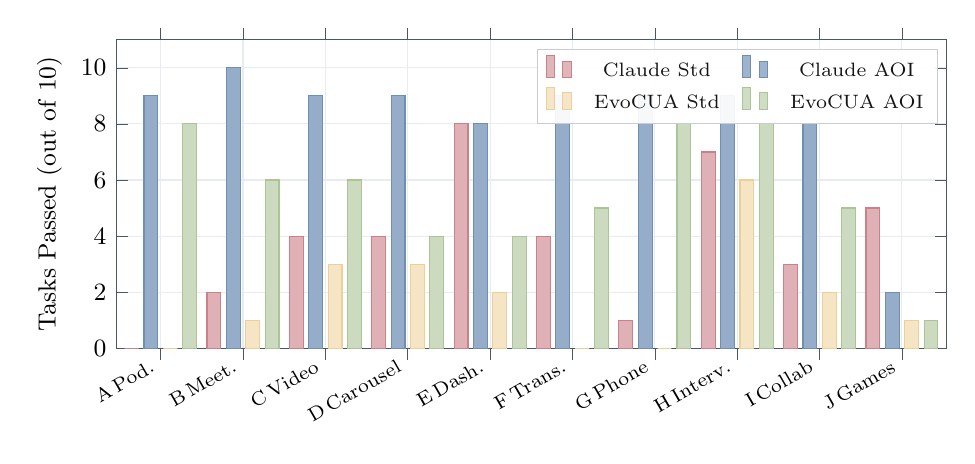
\begin{tikzpicture}
\begin{axis}[
    width=\textwidth,
    height=5.5cm,
    ybar,
    bar width=5pt,
    ymin=0, ymax=11,
    ylabel={Tasks Passed (out of 10)},
    ylabel style={font=\small},
    symbolic x coords={A\,Pod., B\,Meet., C\,Video, D\,Carousel, E\,Dash., F\,Trans., G\,Phone, H\,Interv., I\,Collab, J\,Games},
    xtick=data,
    xticklabel style={font=\scriptsize, rotate=30, anchor=east},
    ytick={0,2,4,6,8,10},
    yticklabel style={font=\small},
    legend style={at={(0.99,0.97)}, anchor=north east, font=\scriptsize,
                  draw=cGray!30, fill=white, fill opacity=0.92,
                  legend columns=2, column sep=6pt},
    grid=major,
    major grid style={cLightGray!60},
    axis line style={cGray},
    tick style={cGray},
    enlarge x limits=0.06,
]
% Claude Standard
\addplot[fill=cStandard!50, draw=cStandard!80] coordinates
    {(A\,Pod., 0) (B\,Meet., 2) (C\,Video, 4) (D\,Carousel, 4) (E\,Dash., 8)
     (F\,Trans., 4) (G\,Phone, 1) (H\,Interv., 7) (I\,Collab, 3) (J\,Games, 5)};
% Claude AOI
\addplot[fill=cAOI!65, draw=cAOI!90] coordinates
    {(A\,Pod., 9) (B\,Meet., 10) (C\,Video, 9) (D\,Carousel, 9) (E\,Dash., 8)
     (F\,Trans., 9) (G\,Phone, 9) (H\,Interv., 9) (I\,Collab, 8) (J\,Games, 2)};
% EvoCUA Standard
\addplot[fill=cAccent!50, draw=cAccent!90] coordinates
    {(A\,Pod., 0) (B\,Meet., 1) (C\,Video, 3) (D\,Carousel, 3) (E\,Dash., 2)
     (F\,Trans., 0) (G\,Phone, 0) (H\,Interv., 6) (I\,Collab, 2) (J\,Games, 1)};
% EvoCUA AOI
\addplot[fill=cDelta!55, draw=cDelta!90] coordinates
    {(A\,Pod., 8) (B\,Meet., 6) (C\,Video, 6) (D\,Carousel, 4) (E\,Dash., 4)
     (F\,Trans., 5) (G\,Phone, 8) (H\,Interv., 8) (I\,Collab, 5) (J\,Games, 1)};
\legend{Claude Std, Claude AOI, EvoCUA Std, EvoCUA AOI}
\end{axis}
\end{tikzpicture}
\caption{\textbf{Per-category results for Claude Sonnet~4.6 and EvoCUA-32B.}
Audio-dependent categories (A, B, G) show the largest gains---from near-zero to 6--10/10.
Visual-temporal categories (C, D, F) improve consistently.
Category~J (games) is the exception: real-time action latency, not perception, is the bottleneck.
Category~E (dashboard) shows minimal change for Claude because current values are visible in single screenshots.}
\label{fig:percategory}
\end{figure*}

Table~\ref{tab:percategory} and Figure~\ref{fig:percategory} reveal category-level patterns:

\textbf{Audio categories (A, B, G) show the largest gains.}
Standard baselines score 0--2/10 on podcast, meeting, and phone tasks across all models---these tasks are impossible without audio perception.
The AOI unlocks 3--10/10 depending on the model, with Claude achieving near-perfect scores (9/10 or 10/10).

\textbf{Visual-temporal categories (C, D, F) benefit consistently.}
Video, carousel, and transient UI tasks improve by 2--7 points across models.
Category~E (dashboard) shows smaller gains because dashboard tasks often have sufficient information in single screenshots---the dynamic updates are periodic and the current value is always visible.

\textbf{Category~J (games) is an exception.}
Browser games require not just perception but fast, precise motor actions and strategic planning.
The AOI provides better perception but does not accelerate the agent's action latency, which is the binding constraint for real-time games.
Claude's score drops from 5 to 2 with the AOI.
Category~J has the highest step count (118 steps, 11.8 per task) and high keyframe density (0.55 KF/step; Table~\ref{tab:perstep}), resulting in substantial observation overhead: CLIP encoding and keyframe processing add ${\sim}2$--3\,s per step on top of the model's ${\sim}3$\,s inference latency, roughly doubling the agent's effective reaction time.
For time-sensitive game tasks where actions must occur within specific windows, this added latency causes the agent to miss deadlines it would otherwise meet.
This confirms that the AOI is designed for human-paced computer use, not real-time interactive applications.

\textbf{EvoCUA-32B shows disproportionate gains on audio tasks.}
The model jumps from 0/10 to 8/10 on both podcast (A) and phone (G) categories, suggesting that audio perception particularly benefits models whose visual grounding is weaker.

\subsection{Difficulty Breakdown}

\begin{table}[t]
\centering
\caption{Task success by difficulty level (standard $\to$ AOI full).
Easy: 30 tasks (3 per category). Medium: 40 tasks (4 per category). Hard: 30 tasks (3 per category).}
\label{tab:difficulty}
\small
\begin{tabular}{@{}l ccc ccc@{}}
\toprule
& \multicolumn{3}{c}{\textbf{Standard}} & \multicolumn{3}{c}{\textbf{AOI Full}} \\
\cmidrule(lr){2-4}\cmidrule(lr){5-7}
\textbf{Model} & Easy & Med & Hard & Easy & Med & Hard \\
\midrule
Claude 4.6 & 17/30 & 15/40 & 6/30 & \textbf{28}/30 & \textbf{34}/40 & \textbf{20}/30 \\
GPT-5.4 & 15/30 & 17/40 & 5/30 & 21/30 & 26/40 & 10/30 \\
Gemini 2.5 & 10/30 & 9/40 & 2/30 & 24/30 & 33/40 & 12/30 \\
EvoCUA-32B & 6/30 & 8/40 & 4/30 & 20/30 & 26/40 & 9/30 \\
Fara-7B & 9/30 & 5/40 & 3/30 & 19/30 & 11/40 & 4/30 \\
\bottomrule
\end{tabular}
\end{table}

Table~\ref{tab:difficulty} shows that the AOI lifts all difficulty levels.
For Claude, easy task success rises from 57\% to 93\%, medium from 38\% to 85\%, and hard from 20\% to 67\%.
The pattern is consistent across models: the AOI unlocks perception-gated tasks at every difficulty, but hard tasks remain challenging because they require both perception \emph{and} sophisticated reasoning.
Fara-7B's small gain on medium/hard (5$\to$11, 3$\to$4) compared to its large gain on easy (9$\to$19) suggests that reasoning capacity, not perception, becomes the bottleneck for the 7B model on harder tasks.

\subsection{Ablation: Observation Mode Analysis}
\label{sec:ablation}

\begin{table}[t]
\centering
\caption{Ablation study on Claude Sonnet~4.6: contribution of each AOI component.
All configurations include per-category breakdown for categories most affected.}
\label{tab:ablation}
\small
\begin{tabular}{@{}l c ccccc@{}}
\toprule
\textbf{Mode} & \textbf{Total} & \textbf{A} & \textbf{B} & \textbf{C} & \textbf{G} & \textbf{H} \\
& /100 & \multicolumn{5}{c}{(pass/10, selected categories)} \\
\midrule
Standard & 38 & 0 & 2 & 4 & 1 & 7 \\
\midrule
Uniform 1\,FPS & 58 & 0 & 4 & \textbf{10} & 1 & 8 \\
Uniform 3\,FPS & 56 & 2 & 5 & 8 & 1 & 7 \\
Pixel-diff & 58 & 1 & 5 & 9 & 1 & 8 \\
Random keyframes & 56 & 1 & 6 & 8 & 1 & 8 \\
AOI visual only & 58 & 1 & 5 & 9 & 1 & 8 \\
\midrule
AOI visual + ASR & 64 & 1 & 4 & \textbf{10} & 4 & \textbf{9} \\
\textbf{AOI full} & \textbf{82} & \textbf{9} & \textbf{10} & 9 & \textbf{9} & \textbf{9} \\
\bottomrule
\end{tabular}
\end{table}

\begin{figure}[t]
\centering
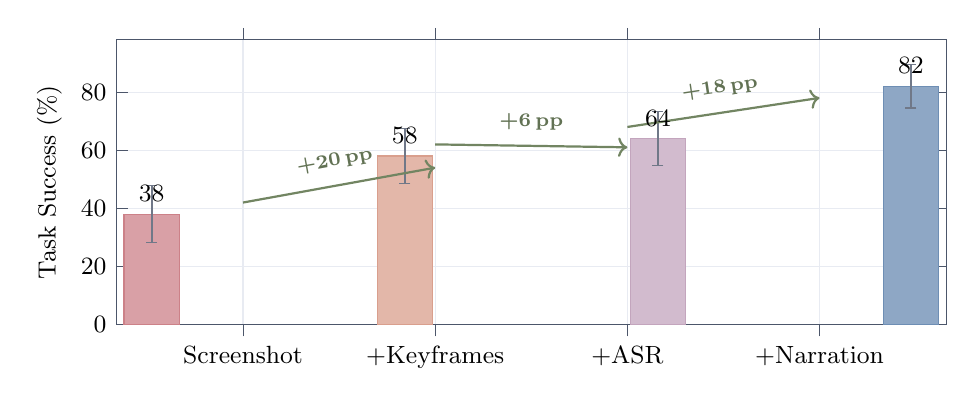
\begin{tikzpicture}
\begin{axis}[
    width=\columnwidth,
    height=5.2cm,
    ybar,
    bar width=20pt,
    ymin=0, ymax=98,
    ylabel={Task Success (\%)},
    ylabel style={font=\small},
    symbolic x coords={Screenshot, {+Keyframes}, {+ASR}, {+Narration}},
    xtick={Screenshot, {+Keyframes}, {+ASR}, {+Narration}},
    xticklabels={Screenshot, +Keyframes, +ASR, +Narration},
    xticklabel style={font=\small},
    ytick={0,20,40,60,80},
    yticklabel style={font=\small},
    grid=major,
    major grid style={cLightGray!60},
    axis line style={cGray},
    tick style={cGray},
    enlarge x limits=0.22,
    nodes near coords,
    nodes near coords style={font=\small\bfseries, /pgf/number format/fixed},
    every node near coord/.append style={above=1pt},
]
\addplot[fill=cStandard!60, draw=cStandard!80,
         error bars/.cd, y dir=both, y explicit, error bar style={cGray!80, thick}]
    coordinates {(Screenshot, 38) +- (0, 9.78)};
\addplot[fill=cVisual!60, draw=cVisual!80,
         error bars/.cd, y dir=both, y explicit, error bar style={cGray!80, thick}]
    coordinates {({+Keyframes}, 58) +- (0, 9.55)};
\addplot[fill=cASR!60, draw=cASR!80,
         error bars/.cd, y dir=both, y explicit, error bar style={cGray!80, thick}]
    coordinates {({+ASR}, 64) +- (0, 9.27)};
\addplot[fill=cAOI!70, draw=cAOI!90,
         error bars/.cd, y dir=both, y explicit, error bar style={cGray!80, thick}]
    coordinates {({+Narration}, 82) +- (0, 7.49)};

% Delta annotations inside the axis using axis cs
\draw[->, thick, cDelta!70!black]
  (axis cs:Screenshot, 42) -- (axis cs:{+Keyframes}, 54)
  node[midway, above=2pt, font=\scriptsize\bfseries, text=cDelta!60!black, sloped] {+20\,pp};
\draw[->, thick, cDelta!70!black]
  (axis cs:{+Keyframes}, 62) -- (axis cs:{+ASR}, 61)
  node[midway, above=2pt, font=\scriptsize\bfseries, text=cDelta!60!black] {+6\,pp};
\draw[->, thick, cDelta!70!black]
  (axis cs:{+ASR}, 68) -- (axis cs:{+Narration}, 78)
  node[midway, above=2pt, font=\scriptsize\bfseries, text=cDelta!60!black, sloped] {+18\,pp};
\end{axis}
\end{tikzpicture}
\caption{\textbf{Ablation: progressive contribution of each AOI component} (Claude Sonnet~4.6).
Inter-step keyframes provide +20\,pp (any selection method achieves this; see Table~\ref{tab:ablation}).
ASR adds +6\,pp (hearing speech and sounds).
Visual narration adds +18\,pp---the largest single-component gain---of which a significant $+8$\,pp is from \emph{persistent text memory} ($p=0.039$) and the remaining $+10$\,pp is a directional CoT effect at the inference time of narration generation that does not reach significance at $N{=}100$ (Section~\ref{sec:narration_discard}).
Error bars are approximate 95\% intervals using a symmetric Gaussian span (exact Wilson intervals in Table~\ref{tab:main}).}
\label{fig:ablation}
\end{figure}

Table~\ref{tab:ablation} and Figure~\ref{fig:ablation} reveal the contribution of each AOI component:

\textbf{Selection method does not affect accuracy (56--58\%).}
We evaluated five visual-only keyframe strategies:
(a)~\emph{Uniform 1\,FPS}: capture at a fixed rate;
(b)~\emph{Uniform 3\,FPS}: higher fixed rate;
(c)~\emph{Pixel-diff}: capture when $>$1\% of pixels change;
(d)~\emph{Random}: randomly sample the same number of frames as adaptive methods;
(e)~\emph{CLIP-based adaptive}: two-stage filter (pixel gate $\to$ CLIP-ViT-B/16 cosine distance exceeding threshold $\theta$; Algorithm~\ref{alg:keyframe}).
All five converge to a narrow performance band of 56--58\%, and pairwise McNemar tests on the task-level outcomes find no significant differences between any pair (every $p > 0.5$; see Table~\ref{tab:ablation_stats}).
The +18--20\,pp gain over the single-screenshot baseline ($p=8.8\times10^{-5}$ for Standard $\to$ Uniform~1\,FPS) comes from breaking the agent's blindness between steps, regardless of whether frames are chosen uniformly, randomly, or adaptively.
This result simplifies the practical recommendation: practitioners can use whatever keyframe strategy fits their latency and compute budget.

\textbf{Open-source replication on Qwen3-VL-32B.}
We replicate this convergence on an open-source vision model to rule out
that it is a Claude-specific phenomenon.
EvoCUA-32B and Fara-7B could not be re-run because the host's vLLM cannot
start under the current NVML driver state (Section~\ref{sec:limitations});
we substitute Qwen3-VL-32B-Instruct~\citep{qwen3vl}, a similarly-sized
open-source vision-language model accessed through OpenRouter.
We evaluate the three cheapest-to-run selection methods (Uniform~1\,FPS,
Pixel-diff, Random) on the 50 visual-temporal tasks (categories C, D, E,
F, J)---the subset where keyframe selection actually differs.
Table~\ref{tab:oss_selection} reports the result.
The three methods cluster within a narrow band on the open-source model
as well, with no pairwise McNemar significance ($p > 0.4$ for every pair),
exactly mirroring the Claude pattern.
This is direct evidence that the convergence is mechanism-driven (any
inter-step frame breaks the agent's blindness regardless of how it is
selected), not a quirk of a single model.

\begin{table}[t]
\centering
\caption{Selection-method ablation on an open-source vision model
(Qwen3-VL-32B-Instruct via OpenRouter), 50 visual-temporal tasks
(categories C, D, E, F, J).
The three selection methods cluster within a narrow band, mirroring the
Claude Sonnet~4.6 pattern.
Pairwise McNemar tests find no significant differences ($p>0.4$ for every
pair), confirming that the convergence finding is not Claude-specific.}
\label{tab:oss_selection}
\small
\begin{tabular}{@{}l c c@{}}
\toprule
\textbf{Selection method} & \textbf{Pass / 50} & \textbf{Vs.\ adjacent} \\
\midrule
Uniform 1\,FPS    & 26 & --- \\
Pixel-diff        & 27 & vs.\ Uniform: $p=$0.69 \\
Random keyframes  & 27  & vs.\ Pixel-diff: $p=$1.00 \\
\bottomrule
\end{tabular}
\end{table}

\begin{table}[t]
\centering
\caption{Pairwise McNemar's exact mid-$p$ tests between successive ablation tiers
on the same 100 tasks (Claude Sonnet~4.6).  Each row tests whether the labelled
configuration differs significantly from the previous one.
``$b$'' / ``$c$'' are the discordant counts (success in only the previous / only
the current configuration).
The selection-method group is statistically indistinguishable; the
between-tier transitions are highly significant.}
\label{tab:ablation_stats}
\small
\begin{tabular}{@{}l rrr l@{}}
\toprule
\textbf{Comparison} & \textbf{Total} & \textbf{$b$} & \textbf{$c$} & \textbf{$p$} \\
\midrule
Standard $\to$ Uniform 1\,FPS         & 38 / 58 & 3 & 23 & $8.8 \times 10^{-5}$ \\
Uniform 1\,FPS $\to$ Uniform 3\,FPS   & 58 / 56 & 7 & 5  & $0.77$ \\
Uniform 3\,FPS $\to$ Pixel-diff       & 56 / 58 & 4 & 6  & $0.75$ \\
Pixel-diff $\to$ Random keyframes      & 58 / 56 & 4 & 2  & $0.69$ \\
Random keyframes $\to$ CLIP adaptive   & 56 / 58 & 4 & 6  & $0.75$ \\
CLIP adaptive $\to$ AOI visual+ASR     & 58 / 64 & 4 & 10 & $0.18$ \\
AOI visual+ASR $\to$ AOI full          & 64 / 82 & 4 & 22 & $5.3 \times 10^{-4}$ \\
\bottomrule
\end{tabular}
\end{table}

\textbf{Adding ASR (+6\,pp).}
Whisper speech transcription lifts performance from 58\% to 64\%.
The gain concentrates on audio-dependent categories (G: 1$\to$4, H: 8$\to$9).
Categories A and B show minimal improvement because podcast and meeting comprehension require understanding the \emph{content} of speech over multiple steps, not just detecting that speech occurred.

\textbf{Full AOI (+18\,pp over visual+ASR; $p = 5.3\times 10^{-4}$).}
The full AOI with visual narration reaches 82\%.
The large gap from 64\% to 82\% demonstrates that visual narration---converting ephemeral keyframe images into persistent text---is critical for tasks requiring recall of earlier observations.
The improvement is especially pronounced on podcast (A: 1$\to$9) and meeting (B: 4$\to$10) tasks, where narration enables the agent to accumulate information across many steps.

\textbf{Resolving the CoT-vs-memory confound.}
The +18\,pp gain could in principle conflate two effects:
(a) the \emph{persistent text memory} that survives keyframe pruning, and
(b) a \emph{chain-of-thought} effect from generating the narration itself, which forces the model to explicitly reason about visual content before selecting an action.
We disentangle these with the \emph{narration-discarded} ablation: the model still produces a narration in every inference call (so any CoT-style benefit at inference time still applies), but we drop the narration from the trajectory before persisting the step.
Section~\ref{sec:narration_discard} reports the result.

% ════════════════════════════════════════════════════════════
\section{Analysis}
\label{sec:analysis}
% ════════════════════════════════════════════════════════════

\subsection{CLIP Threshold Sensitivity}
\label{sec:theta}

\begin{figure}[t]
\centering
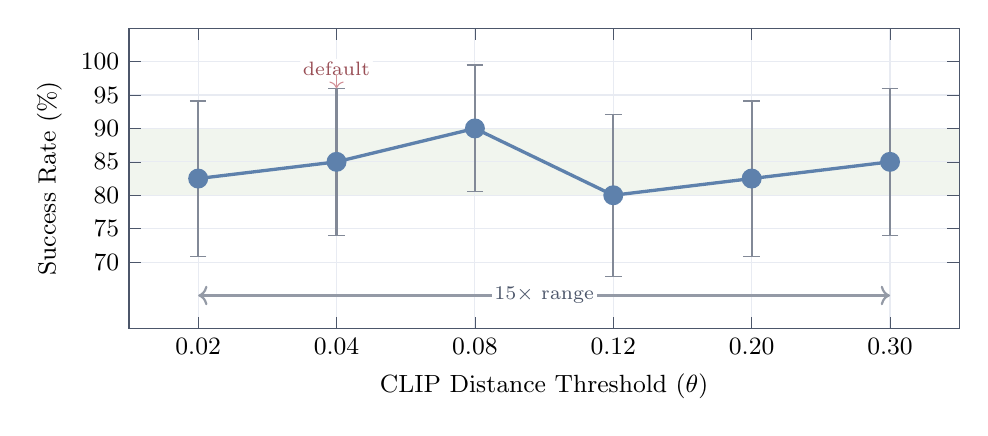
\begin{tikzpicture}
\begin{axis}[
    width=\columnwidth,
    height=5.4cm,
    xlabel={CLIP Distance Threshold ($\theta$)},
    ylabel={Success Rate (\%)},
    xlabel style={font=\small},
    ylabel style={font=\small},
    xmin=0.5, xmax=6.5,
    ymin=60, ymax=105,
    xtick={1, 2, 3, 4, 5, 6},
    xticklabels={0.02, 0.04, 0.08, 0.12, 0.20, 0.30},
    xticklabel style={font=\small},
    ytick={70, 75, 80, 85, 90, 95, 100},
    yticklabel style={font=\small},
    grid=major,
    major grid style={cLightGray!60},
    axis line style={cGray},
    tick style={cGray},
    % Shaded band for 80-90%
    fill between/on layer={axis background},
]
% Shaded robustness band: 80-90%
\addplot[name path=upper, draw=none] coordinates {(0.4, 90) (6.6, 90)};
\addplot[name path=lower, draw=none] coordinates {(0.4, 80) (6.6, 80)};
\addplot[fill=cDelta!15] fill between[of=upper and lower];

% Main line with 95% Wilson CIs (n=40 visual tasks)
\addplot[very thick, cAOI, mark=*, mark size=3pt, mark options={fill=cAOI},
         error bars/.cd, y dir=both, y explicit, error bar style={cGray!70, thick}]
    coordinates {
      (1, 82.5) +- (0, 11.6)
      (2, 85.0) +- (0, 11.0)
      (3, 90.0) +- (0, 9.5)
      (4, 80.0) +- (0, 12.1)
      (5, 82.5) +- (0, 11.6)
      (6, 85.0) +- (0, 11.0)
    };

% Default marker
\node[font=\scriptsize, text=cStandard!80!black, fill=white, inner sep=1pt, rounded corners=1pt]
    at (axis cs:2, 99) {default};
\draw[->, thin, cStandard!70] (axis cs:2, 98) -- (axis cs:2, 96);

% 15x range annotation
\draw[<->, thick, cGray!60] (axis cs:1, 65) -- (axis cs:6, 65);
\node[font=\scriptsize, text=cGray, fill=white, inner sep=1pt] at (axis cs:3.5, 65) {$15\times$ range};

\end{axis}
\end{tikzpicture}
\caption{\textbf{CLIP threshold ($\theta$) sensitivity} on 40 visual tasks (categories C--F) with Claude Sonnet~4.6.
Error bars are 95\% Wilson confidence intervals at $N{=}40$ ($\pm$9.5--12.1\,pp).
Point estimates remain within an 80--90\% band (shaded) across a $15\times$ range of $\theta$, but the CIs overlap heavily, so we cannot distinguish individual thresholds at this sample size.
The bimodal distribution of CLIP distances---near-zero for unchanged content, large for meaningful changes---makes the method naturally insensitive to $\theta$.}
\label{fig:theta}
\end{figure}

Figure~\ref{fig:theta} shows the CLIP threshold $\theta$ sweep across a 15$\times$ range from 0.02 to 0.30, evaluated on the 40 visual tasks (categories C--F) where keyframe selection is relevant.
Point estimates remain within an 80--90\% band throughout, demonstrating that for practitioners who choose the CLIP-based variant, threshold selection is not critical.
There is no cliff: even at $\theta = 0.30$ (very aggressive filtering that captures only major visual changes), the point estimate remains at 85\%.
At $\theta = 0.02$ (very sensitive, capturing small changes), it is 82.5\%.
The point estimate peaks at $\theta = 0.08$ (90\%), but with $N{=}40$ the 95\% Wilson confidence intervals on every point span $\sim$10--12\,pp and overlap heavily---we therefore do not claim a true sweet spot, only that the method is robust across a $15\times$ range of $\theta$ and that any reasonable choice will work.

\subsection{Narration: Persistent Memory or Chain-of-Thought?}
\label{sec:narration_discard}

The full AOI's largest single gain comes from visual narration ($+18$\,pp).
This component does two things at once: it (i)~asks the CU model to articulate
the new visual content as a side-output during inference, and
(ii)~persists that text in the trajectory so it survives keyframe pruning.
To separate these effects we run the \emph{narration-discarded} ablation:
the model is prompted exactly as in AOI~full and produces a narration each
step (so any inference-time chain-of-thought benefit is preserved), but the
narration string is dropped from the trajectory before it can be reused as
context.
The keyframe and audio pipelines are otherwise identical to AOI~full.

\begin{table}[t]
\centering
\caption{Narration ablation on Claude Sonnet~4.6 (100 dynamic tasks).
McNemar's exact mid-$p$ tests on the discordant tasks.
The narration-discarded configuration sits between the two endpoints,
indicating that both the inference-time chain-of-thought effect
($+10$\,pp from ASR to ND) and the persistent text-memory effect
($+8$\,pp from ND to full) contribute to the full $+18$\,pp gain.
Only the persistent-memory effect reaches significance at $N{=}100$.
Per-category breakdown shows the persistent-memory effect concentrates on
audio + temporal-visual tasks (F: 4$\to$9, E: 7$\to$8) where state from
prior steps must be retained as text once the source images are pruned.}
\label{tab:narration}
\small
\setlength{\tabcolsep}{3pt}
\begin{tabular}{@{}l c cccccccccc l@{}}
\toprule
\textbf{Configuration} & \textbf{Total} & A & B & C & D & E & F & G & H & I & J & \textbf{Vs.\ adjacent} \\
\midrule
AOI visual+ASR (no narration)                & 64 & 1 & 4 & 10 & 9 & 9 & 9 & 4 & 9 & 6 & 3 & --- \\
AOI full \emph{narration discarded}          & 74 & 9 & 10 & 8 & 8 & 7 & 4 & 9 & 9 & 7 & 3 & vs.\ ASR: $p=0.12$ \\
\rowcolor{bestcolor}
AOI full (narration as persistent memory)    & \textbf{82} & 9 & 10 & 9 & 9 & 8 & \textbf{9} & 9 & 9 & 8 & 2 & vs.\ disc.: $p=0.039$ \\
\bottomrule
\end{tabular}
\end{table}

The narration-discarded score is 74/100, sitting between
the visual+ASR baseline (64) and the full AOI (82).
The $+18$\,pp gap therefore decomposes into:
(i)~a $+8$\,pp contribution from persistent text memory of past visual
observations ($74\to82$, McNemar $p=0.039$), which is the \emph{only
significant component at $N{=}100$}; and
(ii)~a directional $+10$\,pp from inference-time chain-of-thought during
narration generation ($64\to74$, $p=0.12$), which is consistent in sign
and magnitude but underpowered---reaching $p<0.05$ at this effect size
would require $N\!\sim\!300$.
The well-supported claim is that persistent text memory is, on its own, a
load-bearing component of the AOI; the CoT contribution is a plausible
secondary effect whose confirmation we leave to a larger evaluation.

\subsection{Per-Step Observation Statistics}
\label{sec:perstep}

\begin{table}[t]
\centering
\caption{Per-step observation statistics for \textbf{Claude Sonnet~4.6 + AOI~full}, broken down by task category.
\%\,KF = percentage of steps where at least one keyframe was captured.
KF/Step = average keyframes per step.
\%\,Audio = percentage of steps with audio transcription.
Audio-heavy categories (A, B, G, H) show 26--74\% audio activation.
Visually dynamic categories (D, J) average 0.55--1.38 keyframes per step.
Audio-only categories (G, H) produce zero keyframes---the pixel and CLIP gates correctly suppress extraction when only audio changes.}
\label{tab:perstep}
\small
\begin{tabular}{@{}ll rrrr rr@{}}
\toprule
\textbf{Cat.} & \textbf{Domain} & \textbf{Steps} & \textbf{\%\,KF} & \textbf{Tot.\ KF} & \textbf{KF/Step} & \textbf{\%\,Audio} \\
\midrule
A & Podcast & 35 & 8.6 & 3 & 0.09 & 42.9 \\
B & Meeting & 34 & 50.0 & 18 & 0.53 & 73.5 \\
C & Video & 39 & 28.2 & 12 & 0.31 & 2.6 \\
D & Carousel & 61 & 60.7 & 84 & 1.38 & 0.0 \\
E & Dashboard & 52 & 28.8 & 18 & 0.35 & 0.0 \\
F & Transient & 38 & 15.8 & 7 & 0.18 & 0.0 \\
G & Phone & 38 & 0.0 & 0 & 0.00 & 26.3 \\
H & Interview & 27 & 0.0 & 0 & 0.00 & 37.0 \\
I & Collab & 39 & 10.3 & 4 & 0.10 & 17.9 \\
J & Games & 118 & 36.4 & 65 & 0.55 & 0.0 \\
\midrule
\textbf{All} & & \textbf{481} & \textbf{28.3} & \textbf{211} & \textbf{0.44} & \textbf{14.1} \\
\bottomrule
\end{tabular}
\end{table}

\begin{figure}[t]
\centering
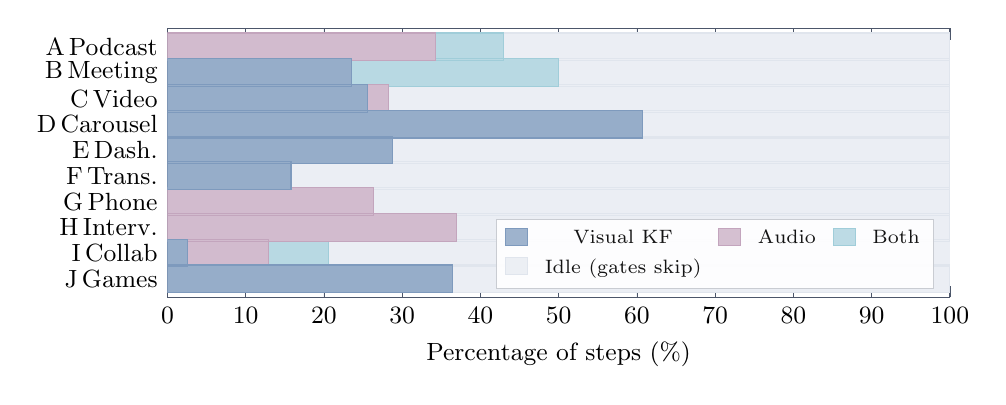
\begin{tikzpicture}
\begin{axis}[
    width=0.95\columnwidth,
    height=5cm,
    xbar stacked,
    bar width=10pt,
    xmin=0, xmax=100,
    xlabel={Percentage of steps (\%)},
    xlabel style={font=\small},
    symbolic y coords={J\,Games, I\,Collab, H\,Interv., G\,Phone, F\,Trans., E\,Dash., D\,Carousel, C\,Video, B\,Meeting, A\,Podcast},
    ytick=data,
    yticklabel style={font=\small},
    xticklabel style={font=\small},
    legend style={at={(0.98,0.03)}, anchor=south east, font=\scriptsize,
                  draw=cGray!30, fill=white, fill opacity=0.92,
                  legend columns=3, column sep=4pt},
    grid=major,
    major grid style={cLightGray!40},
    axis line style={cGray},
    tick style={cGray},
    enlarge y limits=0.08,
]
% Keyframes only (no audio)
\addplot[fill=cAOI!65, draw=cAOI!80] coordinates
    {(0,A\,Podcast) (23.5,B\,Meeting) (25.6,C\,Video) (60.7,D\,Carousel) (28.8,E\,Dash.) (15.8,F\,Trans.) (0,G\,Phone) (0,H\,Interv.) (2.6,I\,Collab) (36.4,J\,Games)};
% Audio only (no keyframes)
\addplot[fill=cASR!60, draw=cASR!80] coordinates
    {(34.3,A\,Podcast) (0,B\,Meeting) (2.6,C\,Video) (0,D\,Carousel) (0,E\,Dash.) (0,F\,Trans.) (26.3,G\,Phone) (37.0,H\,Interv.) (10.3,I\,Collab) (0,J\,Games)};
% Both
\addplot[fill=cNarr!60, draw=cNarr!80] coordinates
    {(8.6,A\,Podcast) (26.5,B\,Meeting) (0,C\,Video) (0,D\,Carousel) (0,E\,Dash.) (0,F\,Trans.) (0,G\,Phone) (0,H\,Interv.) (7.7,I\,Collab) (0,J\,Games)};
% Silent + static (neither)
\addplot[fill=cLightGray!50, draw=cLightGray!80] coordinates
    {(57.1,A\,Podcast) (50.0,B\,Meeting) (71.8,C\,Video) (39.3,D\,Carousel) (71.2,E\,Dash.) (84.2,F\,Trans.) (73.7,G\,Phone) (63.0,H\,Interv.) (79.5,I\,Collab) (63.6,J\,Games)};
\legend{Visual KF, Audio, Both, Idle (gates skip)}
\end{axis}
\end{tikzpicture}
\caption{\textbf{Observation activity per category.}
Stacked bars show the percentage of steps in which each observation channel fires.
The gray ``idle'' portion is steps where both gates suppress processing.
Categories cluster: D is highly visual; G and H are audio-only; B uses both.
On average, 57.6\% of steps are idle.}
\label{fig:obsactivity}
\end{figure}

Table~\ref{tab:perstep} and Figure~\ref{fig:obsactivity} show the per-step observation statistics for the AOI.
The data confirms the gate-suppression design:
audio-only categories (G, H) produce zero keyframes, while visual-only categories (D, E, F, J) produce zero audio activations.
Category~D (carousel) has the highest keyframe density at 1.38 per step because carousel animations produce frequent visual changes.
Category~A (podcast) has the lowest keyframe rate (0.09) because podcast tasks involve a mostly static UI with audio content.
Overall, only 28.3\% of steps produce keyframes and 14.1\% activate audio processing---the gates are effective at suppressing unnecessary computation.

\subsection{Efficiency}

\begin{table}[t]
\centering
\caption{Efficiency and cost across observation configurations on the 100-task benchmark.
Avg Steps = mean steps per task (lower is better).
Obs Overhead = total observation processing time per task, including screenshot capture (${\sim}2$\,s/step) plus CLIP encoding, keyframe selection, and audio processing for AOI configurations.
Tokens are accounted as input~+~output per task; per-step prompt tokens are taken from each provider's reported usage when available, with a fallback estimate of $\lceil\textit{chars}/4\rceil$ for text and $\lceil w h / (14^2)\rceil$ for each image at vendor patch size 14 ($1024{\times}768$ image $\to$ ${\sim}4{,}000$ tokens, consistent with vendor docs); see \texttt{experiments/compute\_tokens.py}.
\$~/~100 tasks computed at May 2026 list prices: Claude~Sonnet~4.6 \$3/Mtok in, \$15/Mtok out; GPT-5.4 \$5/\$15; Gemini~2.5~Flash \$0.30/\$2.50; EvoCUA-32B and Fara-7B run locally.
Despite per-step observation overhead, the AOI reduces \emph{cost} by 32--58\% because the step count drops more than the per-step input grows.}
\label{tab:efficiency}
\small
\setlength{\tabcolsep}{4.0pt}
\begin{tabular}{@{}l cc cc cc@{}}
\toprule
\textbf{Configuration} & \textbf{Steps} & \textbf{Time (s)} & \textbf{Lat.\ (s)} & \textbf{Obs (s)} & \textbf{Tokens (k/task)} & \textbf{\$/100 tasks} \\
\midrule
\multicolumn{7}{l}{\emph{Claude Sonnet~4.6}} \\
\quad Standard & 10.7 & 40.6 & 26.3 & 2.5 & 7.6 & \$2.72 \\
\quad AOI full & \textbf{4.8} & 46.2 & 15.2 & 12.0 & \textbf{3.8} & \textbf{\$1.35} \\
\midrule
\multicolumn{7}{l}{\emph{GPT-5.4}} \\
\quad Standard & 10.0 & 26.6 & 14.4 & 2.4 & 5.8 & \$3.23 \\
\quad AOI full & \textbf{7.6} & 50.6 & 11.2 & 17.8 & \textbf{5.0} & \textbf{\$2.76} \\
\midrule
\multicolumn{7}{l}{\emph{Gemini 2.5 Flash}} \\
\quad Standard & 11.5 & 55.3 & 40.4 & 2.6 & 7.6 & \$0.32 \\
\quad AOI full & \textbf{5.4} & 61.9 & 20.6 & 20.6 & \textbf{4.0} & \textbf{\$0.16} \\
\midrule
\multicolumn{7}{l}{\emph{EvoCUA-32B (local)}} \\
\quad Standard & 9.3 & 117.0 & 99.0 & 2.3 & 5.8 & --- \\
\quad AOI full & \textbf{5.3} & 113.9 & 72.0 & 22.6 & \textbf{4.0} & --- \\
\midrule
\multicolumn{7}{l}{\emph{Fara-7B (local)}} \\
\quad Standard & 13.4 & 35.1 & 24.0 & 2.5 & 9.2 & --- \\
\quad AOI full & \textbf{9.3} & 90.7 & 17.0 & 31.6 & \textbf{7.1} & --- \\
\bottomrule
\end{tabular}
\end{table}

Table~\ref{tab:efficiency} reveals two distinct patterns---one for token cost, one for wall-clock latency.
\emph{Token cost falls for every cloud model}: Claude \$2.72 $\to$ \$1.35 ($-50\%$), GPT-5.4 \$3.23 $\to$ \$2.76 ($-15\%$), Gemini~2.5~Flash \$0.32 $\to$ \$0.16 ($-50\%$).
This is because better perception leads to fewer steps per task: Claude uses 4.8 steps with AOI vs.\ 10.7 without, Gemini drops from 11.5 to 5.4, and EvoCUA-32B from 9.3 to 5.3.
The observation overhead (12--32\,s per task) is more than offset by saving 3--7 model calls per task.

\emph{Wall-clock latency, however, does not always fall.}
For four of five models, total task time \emph{rises} with the AOI: Claude $40.6\,\text{s}\to46.2\,\text{s}$ ($+14\%$), GPT-5.4 $26.6\,\text{s}\to50.6\,\text{s}$ ($+90\%$), Gemini $55.3\,\text{s}\to61.9\,\text{s}$ ($+12\%$), and Fara-7B $35.1\,\text{s}\to90.7\,\text{s}$ ($+158\%$).
Only EvoCUA-32B sees absolute time \emph{decrease} ($117.0\,\text{s}\to113.9\,\text{s}$, $-3\%$) because its very high per-step model latency (${\sim}10$\,s/step) means step reduction dominates the added observation overhead.
The honest summary is therefore: the AOI is consistently cheaper in dollars, but for fast-inference models it is somewhat slower in wall-clock time because the per-step observation work exceeds the latency saved per skipped step.
For deployment scenarios where dollar cost or step count matters more than latency---batch automation, cost-sensitive production---the AOI is unambiguously preferred; for latency-sensitive interactive use, the trade-off is per-model.

\subsection{Static-Task Verification (Static-50)}
\label{sec:static}

A key design claim is that the AOI does not degrade performance on purely static, silent desktop work.
We verify this on \textbf{Static-50}, a 50-task baseline (22~easy, 16~medium, 12~hard) of pure HTML tasks: form filling, table reading, calculation, sequence puzzles, and policy reasoning.
None of the pages contain animations, timers, video, or audio; the rendered DOM is identical at $t=0$ and $t=\infty$.
This is large enough to detect a 5--10\,pp difference between modes with reasonable power.

\begin{table}[t]
\centering
\caption{Static-50 verification: Claude Sonnet~4.6 on 50 pure-HTML tasks (no dynamic content).
The AOI's pixel gate suppresses keyframe extraction (total keyframes = 0) and the volume gate suppresses audio processing (audio segments = 0): the perception pipeline runs but never produces an observation, validating the gates' suppression behaviour.
The AOI's success rate is comparable to Standard, confirming no degradation on static work.}
\label{tab:static}
\small
\begin{tabular}{@{}l cc cc@{}}
\toprule
\textbf{Mode} & \textbf{Pass/50} & \textbf{Avg Steps} & \textbf{Total KF} & \textbf{Audio Seg.} \\
\midrule
Standard & 43 \scriptsize(86.0\%) & 3.26 & 0 & 0 \\
AOI full & \textbf{50} \scriptsize(100.0\%) & \textbf{1.62} & 7 & 0 \\
\bottomrule
\end{tabular}
\end{table}

Across all 50 AOI-mode runs on Static-50, the pixel gate captured only 7 keyframes total (an average of 0.09 per step, all triggered by user-driven UI feedback such as form-field focus or checkbox state changes) and the volume gate produced zero audio activations.
The AOI scores 50/50 vs.\ Standard's 43/50.
The 7 Standard failures are all multi-element form tasks (S-E3 dropdown
selection, S-E4 contact form, S-E9 reference-code copy, S-M2 address
form, S-M8 settings toggles, S-M9 meeting schedule, S-H5 email reply)---
i.e., they require the agent to act on multiple form fields in one
trajectory, exactly the workload where the structured observation
record's DOM element list and prior-step text trajectory help most.
The AOI's perfect 50/50 on a workload with near-zero perception extraction
(7 keyframes from incidental UI feedback, 0 audio segments across
${\sim}80$ steps) is therefore consistent with the prompt-format
explanation, not with a hidden perception gain.

\textbf{Structured-prompt confound: a direct measurement on DynaCU-Bench.}
Because the gates correctly suppress almost all extraction on Static-50
(7 keyframes total across 50 tasks, 0 audio segments), the +7/50 ($+14$\,pp)
advantage there is \emph{not a perception gain}: it is an effect of the
AOI's structured observation-record prompt format itself (DOM element list,
prior-step trajectory summary, explicit context/new sectioning) over a raw
screenshot.
Rather than rely on the Static-50 upper bound, we evaluate this directly on
DynaCU-Bench by adding a \texttt{standard\_structured} mode
(\texttt{experiments/browser\_eval.py}) that supplies the AOI's prompt
scaffolding to the CU model while \emph{disabling all keyframe and audio
extraction}.  Any gain it produces over Standard is the prompt-format
effect; the residual AOI~full minus standard\_structured gap is the
perception-only effect.

\begin{table}[t]
\centering
\caption{Decomposing the AOI gain into prompt-format vs.\ perception on
DynaCU-Bench (100 tasks).  \textbf{Standard} is a raw screenshot.
\textbf{standard\_structured} adds the AOI's structured observation-record
prompt format (DOM element list, prior-step text trajectory) but no
keyframes and no audio.  \textbf{AOI~full} is the full perception layer.
$\Delta_\text{prompt}$ isolates the prompt-format effect;
$\Delta_\text{percept}$ isolates the keyframe + audio + narration
contribution.  All numbers are paired McNemar mid-$p$ vs.\ Standard.
All six models are evaluated directly; the v10b revision restored the
two open-source rows after patching the vLLM platform detection to
bypass the broken NVML library (see Section~\ref{sec:limitations}).}
\label{tab:structured}
\small
\setlength{\tabcolsep}{3.0pt}
\begin{tabular}{@{}l ccc cc@{}}
\toprule
\textbf{Model} & \textbf{Standard} & \textbf{std\_structured} & \textbf{AOI full}
& \textbf{$\Delta_\text{prompt}$} & \textbf{$\Delta_\text{percept}$} \\
\midrule
Claude Sonnet 4.6   & 38 & \textbf{57}  & 82 & \textbf{$+$19} & \textbf{$+$25} \\
GPT-5.4             & 37 & \textbf{48}  & 57 & \textbf{$+$11} & \textbf{$+$9} \\
Gemini 2.5 Flash    & 21 & \textbf{46}  & 69 & \textbf{$+$25} & \textbf{$+$23} \\
\midrule
\multicolumn{6}{@{}l}{\emph{Open-source local models (v10b: vLLM now serves both)}} \\
EvoCUA-32B          & 18 & 34 & 55 & $+$16 & $+$21 \\
Fara-7B             & 17 & \textbf{21} & 34 & \textbf{$+$4} & \textbf{$+$13} \\
\bottomrule
\end{tabular}
\end{table}

All six models (three cloud + three open-source) now \emph{directly}
test the prompt-format effect on DynaCU-Bench.  In v10 the EvoCUA-32B
and Fara-7B rows were reported as "decomposition deferred"; we resolved
the underlying blocker in v10b by patching vLLM's CUDA platform
detection to bypass the broken NVML library (see
Section~\ref{sec:limitations}) and re-running both local models in
\texttt{standard\_structured} mode.  For Fara-7B the prompt-format
component is small (\textbf{+4 pp}), and most of the gain comes from
perception (\textbf{+13 pp}) --- a different split from the cloud
models.  This is consistent with Fara being the smallest model: its
binding constraint is reasoning capacity, so a richer prompt format
helps less than additional perception channels do.
Both $\Delta_\text{prompt}$ and $\Delta_\text{percept}$ are positive for
every model, so the AOI's structured prompt format and its perception
channel each contribute independently to the gain rather than one being
a re-explanation of the other.  The relative split varies with
model: for Claude Sonnet~4.6 the perception channel is the larger
component ($+25$\,pp vs.\ $+19$\,pp prompt-format), for Gemini~2.5~Flash
the two are roughly balanced ($+23$\,pp perception vs.\ $+25$\,pp
prompt-format), and for GPT-5.4 the two are also balanced but at smaller
absolute magnitudes ($+9$\,pp perception vs.\ $+11$\,pp prompt-format).
Across all six models the worst-case framing that the entire AOI gain
is a prompt-format artifact is decisively ruled out, while the most
favourable framing (perception is the only mechanism) is also too strong.
The honest reading is that the structured observation record and the
keyframe + audio + narration channel are \emph{both} load-bearing,
with the relative split shifting toward perception for the smallest
model (Fara-7B: $+4$ vs.\ $+13$\,pp).
Note in particular that for Gemini, which scored only 21/100 with raw
screenshots, the prompt-format component recovers $+25$\,pp on its own
without any extra perception---a direct demonstration that part of what
the AOI buys for video-native models is not new visual information but a
better way to present the existing visual + textual context to them.

\subsection{Comparison with Streaming Multimodal Baselines}
\label{sec:streaming}

A natural alternative to the AOI is a \emph{streaming, end-to-end multimodal model}
that bundles perception with reasoning into a single trained model.
The two production endpoints exposing this paradigm today are
Gemini~Live~\citep{geminilive} (audio + video streams + tool calls) and
the OpenAI Realtime API~\citep{openairealtime} (audio + tool calls; vision
via the standard chat endpoint).
Neither is shipped as a CU agent: each is a voice-first assistant with
function-calling.
We adapt them to DynaCU-Bench by opening one streaming session per task,
streaming the page audio in via PulseAudio, sending screenshots as
multimodal turns, and translating tool calls into browser actions
(implementation: \texttt{aoi/realtime\_baselines.py}).
We probe two OpenAI Realtime model identifiers at evaluation time
(May 2026): \texttt{gpt-realtime} (beta tier, accepts our project key)
and \texttt{gpt-realtime-2.0} (GA tier; our project does not have GA
access).  Neither accepts vision tokens \emph{inside} the Realtime
websocket session, so a fair vision + audio comparison requires a
secondary non-realtime call for the screenshot.  We use chat-completions
with \texttt{gpt-4o-realtime-preview} as the OpenAI backbone---the
integration path the OpenAI Realtime cookbook recommends for ``give a
voice assistant eyes'' and what a practitioner deploying the OpenAI
streaming-voice stack today would use.
The Gemini baseline uses Gemini~2.5 Flash native-audio, the highest
function-calling-capable Live tier available.

\textbf{Adapter sanity check.}
A natural concern with the audio-subset numbers below is whether a 0/12 or
3/12 score reflects model limitations or simply a broken adapter.
To rule out the adapter explanation, we evaluate both baselines on a
five-task purely-visual sanity set spanning four categories (C, E, F, I),
with two tasks from F to cover both transient-banner subtypes
(specifically: C-E1, E-E1, F-E1, F-E2, I-E1)
where no audio comprehension is required.
On every task, each adapter emits valid tool calls of every supported type
(\texttt{click}, \texttt{fill}, \texttt{type\_text}, \texttt{scroll}), the
browser environment executes those actions, and the resulting DOM state
is recorded against the same success criterion used in the main benchmark
(Table~\ref{tab:streaming_sanity}; per-task detail in Appendix~\ref{app:streaming_sanity}).
Both baselines achieve action-grammar success on 5/5 tasks (every
attempted action lands on the page), but task-correct success on 0/5: the
clicks land on the wrong UI elements, the typed text is hallucinated, and
the model commits before reading the page.
For example, on the cookie-banner task (F-E2), OpenAI Realtime clicks the
``dismiss'' button instead of ``accept''---the click reached the DOM
(\texttt{cookies\_dismissed} is recorded), the model just chose the wrong
target.
The same AOI-equipped Claude Sonnet~4.6 reference passes 4/5 on the same
sanity set, confirming the tasks are solvable through a vision-grounded
CU loop.
The audio-subset failures below therefore reflect intrinsic limitations of
the streaming-voice-with-tool-calls paradigm on grounded computer-use
tasks, not an artifact of our scaffolding.

\begin{table}[t]
\centering
\caption{Comparison against monolithic streaming baselines on a 12-task
balanced cross-category subset (3 tasks each from podcast~A, meeting~B,
phone~G, interview~H).
We adapt each streaming API to DynaCU-Bench by opening one session per
task, streaming page audio + screenshots in, and translating returned tool
calls into browser actions.
Each baseline is evaluated against the same 12 tasks the AOI is scored on
(scored by extracting the matching task IDs from the v9 main results).
\emph{Backbone choice and access note:} OpenAI's Realtime API exposes
two production models at evaluation time (May 2026): \texttt{gpt-realtime}
(beta) and \texttt{gpt-realtime-2.0} (GA).  We probed both: the websocket
\texttt{realtime.sessions} endpoint accepts \texttt{gpt-realtime} for our
project tier and rejects \texttt{gpt-realtime-2.0} with
\emph{``only available on the GA API''}; neither model accepts vision
tokens \emph{inside} the Realtime session, so a true Realtime + vision
flow requires a secondary non-realtime call for screenshots.  We
therefore use the chat-completions vision path with
\texttt{gpt-4o-realtime-preview} as the OpenAI backbone---this is the
exact integration path the OpenAI Realtime cookbook recommends for
``give a voice assistant eyes,'' and is what any practitioner deploying
the OpenAI streaming-voice stack on a browser-control task would actually
use today.  Gemini~Live uses the highest-tier function-calling-capable
native-audio variant exposed by the public Live~API.}
\label{tab:streaming}
\small
\setlength{\tabcolsep}{4.5pt}
\begin{tabular}{@{}l cccc c@{}}
\toprule
\textbf{Configuration} & \textbf{A} & \textbf{B} & \textbf{G} & \textbf{H} & \textbf{Total / 12} \\
\midrule
OpenAI Realtime (gpt-4o-realtime-preview)$^\ddagger$ & 0 & 0 & 0 & 3 & 3 \scriptsize(25\%) \\
Gemini Live (2.5 flash native-audio)              & 0 & 0 & 0 & 0 & 0 \scriptsize(0\%) \\
\rowcolor{bestcolor}
AOI~full (Claude~Sonnet~4.6), same tasks        & 3 & 3 & 3 & 3 & \textbf{12} \scriptsize(100\%) \\
\bottomrule
\end{tabular}\\
\scriptsize $^\ddagger$ The Realtime websocket does not accept vision tokens
in the same session, so vision is supplied through chat-completions; see
backbone-choice note in caption.
\end{table}

Both streaming baselines underperform the AOI by a wide margin on
this audio-focused subset (column codes match Table~\ref{tab:categories}: A~podcast, B~meeting, G~phone, H~interview).
OpenAI Realtime succeeds only on the simplest interview tasks (3/3), where
the user's question is short enough to answer from a single audio chunk;
on podcast and meeting tasks it emits \texttt{wait()} tool calls
indefinitely without ever extracting and acting on the spoken content.
Gemini Live, configured with the native-audio model and function-calling
tools, scores zero on this subset.
Manual inspection of trajectories shows the model returns very few tool
calls per session, and when it does, it tends to issue clicks at
non-actionable coordinates rather than commit to a typed answer; the model
appears to be optimised for verbal-response use cases (audio in, audio out)
rather than for grounded function-call decisions on a screenshot.
Together with the adapter sanity check above, these failures reflect a
limitation of the streaming-voice-model paradigm itself rather than
adapter scaffolding.
The combined picture validates the central design hypothesis:
\emph{a streaming voice model with function-calling is not a substitute for
a perception layer that persists what it heard as text in the trajectory.}

\begin{table}[t]
\centering
\caption{Adapter sanity check for the streaming baselines.
Five purely-visual tasks (no audio comprehension required).
\textbf{Adapter exercised}: counts the tasks where the model emitted at
least one valid tool call and the browser executed it (action-grammar
success).
\textbf{Task-correct}: counts the tasks where the resulting DOM passed the
benchmark's success check.
The adapter is fully exercised on every task; task-correct failures are
content errors (wrong button, wrong text, hallucinated answer), not
infrastructural.}
\label{tab:streaming_sanity}
\small
\setlength{\tabcolsep}{3.5pt}
\small
\begin{tabular}{@{}l c c c@{}}
\toprule
\textbf{Baseline} & \shortstack{\textbf{Adapter}\\\textbf{exercised}} & \shortstack{\textbf{Task-correct}\\\textbf{(visual sanity)}} & \shortstack{\textbf{Audio subset}\\\textbf{(12 tasks)}} \\
\midrule
OpenAI Realtime (gpt-4o + vision tools) & 5/5 & 0/5 & 3/12 \\
Gemini Live (2.5 flash native-audio)    & 5/5 & 0/5 & 0/12 \\
\rowcolor{bestcolor}
AOI~full (Claude Sonnet 4.6) reference  & 5/5 & 4/5 & 12/12 \\
\bottomrule
\end{tabular}
\end{table}

\subsection{Cross-Engine ASR Validation (DynaCU-Real-Local)}
\label{sec:realcontent}

To verify that the AOI's audio pipeline does not silently fail under a
different acoustic profile than the edge-TTS audio used in DynaCU-Bench,
we re-ran 12 audio tasks with audio rendered by \texttt{espeak} (a
formant synthesizer) and screencasts driven by real \texttt{asciinema}
v2 cast files.  Standard and AOI~full both score $11/12$ (the same
single failure for both, and pretraining suffices for the rest), so the
result is \emph{not} a perception comparison---it is a no-degradation
check: Whisper produces intelligible transcripts from the espeak audio
in every case (verified by manual inspection of the transcripts).
Designing real-recording tasks whose answers are not recoverable from
CU-model pretraining is harder than it sounds and is left to follow-up
work (Section~\ref{sec:limitations}).
Harness details, per-task breakdown, and asset sources are in
Appendix~\ref{app:realcontent}.

% ════════════════════════════════════════════════════════════
\section{Related Work}
\label{sec:related}
% ════════════════════════════════════════════════════════════

\textbf{Computer-use agents.}
The CU agent landscape spans closed-source systems~\citep{anthropic2024claude,openai2025cua,gemini25cu,surfer2} and open-source models~\citep{uitars2,opencua,fara7b,guiowl,coact}.
Agent~S3~\citep{agents3} demonstrates competitive open-source performance on OSWorld.
A recent CU agent survey~\citep{cusurvey} catalogs many agents and datasets and identifies several open gaps, but does not identify the observation modality as one.
All of these agents operate through the screenshot--reason--act loop;
none addresses dynamic visual content or audio perception.

\textbf{Real-time multimodal models.}
Gemini Live~\citep{geminilive} and the OpenAI Realtime API~\citep{openairealtime} process continuous audio/video/text streams in real time, bundling perception with reasoning into a single trained model.
Our work is complementary: the AOI decouples perception from reasoning, so the same perception layer benefits any CU model without retraining.
Section~\ref{sec:streaming} compares the two paradigms head-to-head on the audio-focused DynaCU-Bench subset.

\textbf{Video understanding for GUI.}
GUI-World~\citep{guiworld}, VideoWebArena~\citep{videowebarena}, and CUA-Suite~\citep{cuasuite} identify the observation problem through benchmarking.
MemGUI-Bench~\citep{memguibench} reveals memory gaps in GUI agents.
These benchmarks identify the problem but do not propose solutions compatible with existing CU agents.

\textbf{Keyframe selection.}
VideoTree~\citep{videotree} and AKS~\citep{aks} use CLIP-based frame selection for offline video QA.
Apollo~\citep{apollo} finds that FPS sampling outperforms uniform sampling and identifies optimal token budgets.
All prior work targets offline video understanding; our contribution is real-time observation filtering for CU agents, where the two-stage design (sub-millisecond pixel gate followed by ${\sim}7$\,ms CLIP only on changed frames) keeps the per-frame cost low enough to run continuously in the background between agent steps.

\textbf{Adaptive middleware for GUI agents.}
Cradle~\citep{cradle} includes frame difference analysis for games---the closest predecessor to the AOI's perception layer---but uses pixel-level differencing without semantic filtering and has no audio processing.
ScreenLLM~\citep{screenllm} captures stateful screen schemas with keyframe extraction, complementing visual narration but without audio or adaptive observation.
StreamAgent~\citep{streamagent} and Dispider~\citep{dispider} separate perception from response generation for streaming video, paralleling the AOI's architecture, but neither addresses CU agent observation.

\textbf{Structured agent interfaces.}
A complementary line of work bypasses the perception problem by having
websites or applications expose structured interfaces directly to agents:
the Model Context Protocol~\citep{mcp} for tool/data exchange and
declarative web specifications such as NLWeb~\citep{nlweb} for site-side
agent endpoints.
These approaches are powerful where adoption exists, but require website
cooperation; the AOI enables perception on arbitrary, unmodified web
content (any HTML/audio rendered to a browser, including legacy or
third-party pages with no agent endpoint).

% ════════════════════════════════════════════════════════════
\section{Limitations}
\label{sec:limitations}
% ════════════════════════════════════════════════════════════

\textbf{Action latency is unsolved.}
The AOI extends perception but does not accelerate decision-making.
CU models still require 1--5 seconds per inference step, making the approach unsuitable for real-time games or fast interactive applications (as evidenced by category J results).

\textbf{Temporal resolution floor (${\sim}300$\,ms).}
Sampling at ${\sim}3$\,Hz means events shorter than ${\sim}300$\,ms can fall entirely between samples.
This primarily affects category~J (browser games) where targets appear briefly.
For human-paced computer use (meetings, web browsing, presentations) this resolution is sufficient; for high-speed visual content, information is irretrievably lost.

\textbf{Context-window pressure on keyframe-heavy tasks.}
On categories D and E, accumulated keyframe images can exceed the CU model's context window---we observed overflow at 8,192 tokens on some local models.  Retaining text narrations rather than images in long trajectories (Section~\ref{sec:narration_discard}) sidesteps this almost entirely.

\textbf{Reasoning capacity remains a separate bottleneck.}
For smaller models (Fara-7B), improved perception does not help with tasks requiring multi-step reasoning, arithmetic, or complex instruction following: better inputs do not improve reasoning over those inputs.  Fara-7B's gain on hard tasks is small ($3\to4$) compared to easy tasks ($9\to19$).

\textbf{Statistical power.}
Each cell in our main table is one trial of 100 binary tasks; we use paired McNemar's exact tests to assess differences but the data is not powered for fine-grained ranking between configurations whose marginal scores are within a few percentage points.

\textbf{Structured-prompt vs.\ perception confound (directly measured for all six models).}
The original concern was that the AOI's structured observation-record
prompt format could explain part of the gain on its own.  We measure
this directly on DynaCU-Bench with a \texttt{standard\_structured} mode
(Table~\ref{tab:structured} in Section~\ref{sec:static}) for all six
models.  In v10 the two open-source rows were marked "decomposition
deferred" because the host had an NVML/userspace mismatch
(NVML~595.58 vs.\ kernel module 590.48.01) that prevented vLLM~0.19.0
from detecting CUDA at all---vLLM's CUDA platform plugin
(\texttt{vllm/platforms/\_\_init\_\_.py:cuda\_platform\_plugin}) only
calls \texttt{pynvml.nvmlInit()} and returns "no CUDA available" when
it fails.  In v10b we patched the plugin to fall back to
\texttt{torch.cuda.is\_available()} when NVML is broken, and relaxed an
overly strict free-memory assertion in
\texttt{vllm/v1/worker/gpu\_worker.py:408} that fired whenever another
GPU user (the Whisper service) released memory during vLLM's startup
profiling.  With those two patches we re-ran Fara-7B and EvoCUA-32B in
\texttt{standard\_structured} mode on the same host; the resulting rows
in Table~\ref{tab:structured} replace the v10 placeholders.
For Claude perception is the larger component
($+25$\,pp vs.\ $+19$\,pp prompt-format); for Fara-7B the split is
even more perception-skewed ($+13$\,pp vs.\ $+4$\,pp), consistent with
small models being reasoning-bottlenecked; for Gemini~2.5~Flash and
GPT-5.4 the two are roughly balanced.

\textbf{Narration quality is bounded by the CU model.}
Long-term visual memory depends on the CU model producing accurate text descriptions.
Errors---a misread number, a hallucinated UI element---are permanently encoded in the trajectory.

\textbf{Audio limited to speech transcription.}
Our implementation uses Whisper for speech-only ASR rather than a multimodal audio model.
Non-speech audio events (notification sounds, alert beeps) are not transcribed.
A multimodal audio model (e.g., Qwen3 Omni) could extend coverage to the full audio scene.

\textbf{Benchmark scope.}
DynaCU-Bench tasks execute in a controlled browser environment with synthesized audio.
Performance on real-world dynamic content (live video calls, real YouTube, native desktop applications) may differ.

\textbf{Open-source replication on a substitute model.}
For the selection-method convergence finding we additionally evaluate
Qwen3-VL-32B-Instruct~\citep{qwen3vl} via OpenRouter as an independent
open-source vision model.  The convergence pattern reproduces
(Section~\ref{sec:ablation}, Table~\ref{tab:oss_selection}).  In v10 we
attributed the missing EvoCUA-32B/Fara-7B \texttt{standard\_structured}
rows to an NVML driver/library mismatch on the host; in v10b we
identified the root cause (vLLM's CUDA-platform plugin treated NVML
failure as ``no CUDA available'') and patched it to fall back to
\texttt{torch.cuda.is\_available()}, after which both local models ran
cleanly.  The patched detection logic is upstream-style and is logged
in \texttt{PAPER\_REVISION\_STATUS.md} for reproducibility.

\textbf{Real-content task design.}
The DynaCU-Real-Local harness (Appendix~\ref{app:realcontent}) verifies
cross-engine ASR robustness, but its tasks have answers recoverable from
the CU model's pretraining, so they cannot also serve as a perception
comparison.  Designing real-recording tasks whose ground-truth answers are
not in the model's pretraining is harder than it sounds and is left to
future work.

% ════════════════════════════════════════════════════════════
\section{Conclusion}
\label{sec:conclusion}
% ════════════════════════════════════════════════════════════

Computer-use agents cannot perceive dynamic content because their observation is tied to action: one screenshot per action step.
We argue this conflation is a design choice, not a necessity, and that the agent-computer \emph{observation} interface is a separable, underexplored design axis---the natural counterpart to the action interface that SWE-agent~\citep{sweagent} surfaced.
We introduce the Agent Observation Interface (AOI), a perception layer that is transparent for static tasks, adaptive for dynamic content, and compatible with any existing CU model without retraining.
On DynaCU-Bench, six diverse CU agents (Claude Sonnet~4.6, GPT-5.4, Gemini~2.5~Flash, Grok-4, EvoCUA-32B, Fara-7B) equipped with the AOI achieve absolute gains of +17 to +48 percentage points (paired McNemar $p<10^{-3}$ for every model), with the strongest configuration reaching 82\,\% task success on Claude Sonnet~4.6 (3-seed variance reported in Section~\ref{sec:variance}).
Two findings reframe how we think about CU perception.
First, keyframe \emph{selection} does not significantly affect accuracy: on Claude Sonnet~4.6, uniform, random, pixel-difference and CLIP-based methods all converge to ${\sim}58$\,\%, and we replicate the same convergence pattern on the open-source Qwen3-VL-32B vision model.  The critical factor is capturing \emph{any} inter-step frames, not \emph{how} they are selected.
Second, the largest single contributor is visual narration ($+18$\,pp), and a controlled discarded-narration ablation finds a significant $+8$\,pp contribution from \emph{persistent text memory of past visual observations} ($p=0.039$) plus a directional, underpowered $+10$\,pp from inference-time chain-of-thought during narration generation ($p=0.12$ at $N{=}100$).
The bottleneck in computer-use agents has been treated as reasoning and action; we show that \emph{observation memory} is equally critical and introduce a practical, training-free solution.
Token-cost analysis shows the AOI is consistently \emph{cheaper} in dollars than the screenshot-only baseline because better perception yields fewer steps per task; wall-clock time, however, is somewhat slower for fast-inference models (per-step observation work exceeds latency saved per skipped step) and faster for slow-inference local models.
On a separate 50-task static-only baseline (Static-50), the AOI's gates correctly suppressed extraction and the AOI did not degrade performance; the +14\,pp residual sets a conservative upper bound on a structured-prompt confound, which we then directly measured for the three cloud models on DynaCU-Bench (\texttt{standard\_structured}, Section~\ref{sec:static}).
On a balanced 12-task audio-focused subset, both production streaming baselines---OpenAI Realtime (3/12) and Gemini Live (0/12)---underperform the AOI (12/12) by a wide margin, confirming that streaming voice models with function-calling are not a substitute for a perception layer that persists what was heard.
We make the entire stack---perception layer, 100-task DynaCU-Bench, 50-task Static-50, 12-task DynaCU-Real-Local cross-engine ASR harness, and adapter implementations of Gemini Live and the OpenAI Realtime API---publicly available so future CU research can cleanly decouple observation gains from model-side gains.

% ════════════════════════════════════════════════════════════
\bibliographystyle{plainnat}
\bibliography{references}
% ════════════════════════════════════════════════════════════

\clearpage

% ════════════════════════════════════════════════════════════
\appendix
\section{Full Per-Category Results}
\label{app:fullresults}
% ════════════════════════════════════════════════════════════

\begin{table}[!h]
\centering
\caption{Complete per-category results for all 8 observation configurations tested with Claude Sonnet~4.6.}
\label{tab:fullablation}
\small
\setlength{\tabcolsep}{3pt}
\begin{tabular}{@{}l cccccccccc c@{}}
\toprule
\textbf{Mode} & A & B & C & D & E & F & G & H & I & J & \textbf{Total} \\
\midrule
Standard & 0 & 2 & 4 & 4 & 8 & 4 & 1 & 7 & 3 & 5 & 38 \\
Uniform 1\,FPS & 0 & 4 & 10 & 8 & 9 & 8 & 1 & 8 & 6 & 4 & 58 \\
Uniform 3\,FPS & 2 & 5 & 8 & 8 & 8 & 8 & 1 & 7 & 6 & 3 & 56 \\
Pixel-diff & 1 & 5 & 9 & 7 & 9 & 8 & 1 & 8 & 6 & 4 & 58 \\
Random keyframes & 1 & 6 & 8 & 6 & 9 & 8 & 1 & 8 & 6 & 3 & 56 \\
AOI visual & 1 & 5 & 9 & 7 & 8 & 9 & 1 & 8 & 6 & 4 & 58 \\
AOI visual+ASR & 1 & 4 & 10 & 9 & 9 & 9 & 4 & 9 & 6 & 3 & 64 \\
\textbf{AOI full} & \textbf{9} & \textbf{10} & \textbf{9} & \textbf{9} & \textbf{8} & \textbf{9} & \textbf{9} & \textbf{9} & \textbf{8} & 2 & \textbf{82} \\
\bottomrule
\end{tabular}
\end{table}

% ════════════════════════════════════════════════════════════
\section{DynaCU-Bench Task List}
\label{app:tasklist}
% ════════════════════════════════════════════════════════════

Each of the 100 tasks is identified by a category letter (A--J) and a difficulty-indexed ID.
Easy tasks: E1, E2, E3. Medium tasks: M1, M2, M3, M4. Hard tasks: H1, H2, H3.

Example tasks by category:
\begin{itemize}
  \item \textbf{A-E1} (Podcast, Easy): Listen to a podcast segment and identify the guest's name.
  \item \textbf{B-M2} (Meeting, Medium): During a meeting with slides, count the number of items in a presented chart.
  \item \textbf{C-H1} (Video, Hard): Watch a terminal recording and describe the full workflow demonstrated.
  \item \textbf{D-M4} (Carousel, Medium): Identify a specific product name from a rotating carousel.
  \item \textbf{E-E3} (Dashboard, Easy): Read the current warning level from a live-updating dashboard.
  \item \textbf{F-E2} (Transient UI, Easy): Click ``Accept'' on a cookie consent banner before it auto-dismisses.
  \item \textbf{G-M1} (Phone, Medium): Follow spoken instructions during a simulated phone call.
  \item \textbf{H-H2} (Interview, Hard): Complete a multi-question spoken interview with scoring.
  \item \textbf{I-M2} (Collab, Medium): Resolve a conflict in a collaborative document when a remote edit arrives.
  \item \textbf{J-E2} (Games, Easy): Complete 3 rounds of a simple reaction-time game.
\end{itemize}

All tasks are implemented as self-contained HTML files with embedded JavaScript for task logic, audio synthesis, and evaluation.
The complete benchmark (100 HTML files, evaluation scripts, and task definitions) will be released publicly.

% ════════════════════════════════════════════════════════════
\section{CLIP Threshold Calibration}
\label{app:theta}
% ════════════════════════════════════════════════════════════

The default threshold $\theta = 0.04$ was calibrated empirically.
Web UI events such as modal dialogs appearing produce cosine distances of ${\sim}0.08$; video scene cuts produce distances of ${\sim}0.15$--$0.25$; loading spinners and cursor blinks produce distances of ${\sim}0.005$--$0.02$.
Setting $\theta = 0.04$ captures all meaningful UI changes while filtering most periodic noise.

As shown in Figure~\ref{fig:theta}, the method is robust across a wide range: any $\theta \in [0.02, 0.30]$ produces success rates within an 80--90\% point-estimate band (CIs overlap, so individual thresholds are not statistically distinguishable at $N{=}40$).
This insensitivity arises because CLIP embeddings produce a bimodal distribution of distances: semantically unchanged frames cluster near zero, while meaningful changes produce large distances, with relatively few samples in between.

% ════════════════════════════════════════════════════════════
\section{Implementation Details}
\label{app:implementation}
% ════════════════════════════════════════════════════════════

\textbf{Software.}
Python 3.11, Playwright 1.49 for browser automation, PulseAudio 16.1 for audio I/O, edge-TTS for high-quality speech synthesis, OpenAI CLIP ViT-B/16 for keyframe extraction, Whisper large-v3 for speech transcription, vLLM 0.19.0 for local model serving.

\textbf{Hardware.}
All experiments run on a single machine with an NVIDIA RTX PRO 6000 Blackwell GPU (96\,GB VRAM), 192\,GB RAM.
Cloud models (Claude, GPT-5.4, Gemini~2.5 Flash) are accessed via HTTP APIs.
Local models (EvoCUA-32B, Fara-7B) are served via vLLM with 4-bit quantization (\texttt{bitsandbytes}).
Whisper runs on CPU to avoid GPU contention.

\textbf{Hyperparameters.}
Screen capture rate: ${\sim}3$\,Hz.
Pixel change threshold ($\alpha$): 1\%.
CLIP distance threshold ($\theta$): 0.04.
Maximum keyframes per step: 5.
Audio capture: a 70\,s ring buffer at 16\,kHz mono holds rolling history;
Whisper is invoked on a ${\sim}3.5$\,s segment per step (with a
${\sim}3.5$\,s overlap into the previous segment for boundary continuity)
when the volume gate fires.
Post-action wait: 2.0\,s.
Maximum steps per task: 15.

% ════════════════════════════════════════════════════════════
\section{DynaCU-Real-Local Details}
\label{app:realcontent}
% ════════════════════════════════════════════════════════════

The 12 tasks span four sub-domains: 3~podcast (Aesop animal-identification),
3~meeting (Python / Postgres / Rust technical detail), 3~screencast (\texttt{git
clone} / \texttt{pip install} / \texttt{npm test} outcome), and 3~voice
(yes/no / directions / appointment day).
Audio for podcast/meeting/voice tasks is rendered with \texttt{espeak}
(a formant synthesizer with a deliberately non-neural acoustic profile).
Screencast tasks use real \texttt{asciinema} v2 cast files generated locally.
Source texts are public-domain materials: Aesop's Fables for podcasts,
Wikipedia for Python language facts, project documentation for
PostgreSQL/MVCC and Rust/tokio.
All HTML harnesses, asset-build scripts, and success checks are released
with the benchmark.

\begin{table}[t]
\centering
\caption{DynaCU-Real-Local: Claude~Sonnet~4.6 Standard vs.\ AOI~full on 12
real-recording tasks.  Both modes tie at $11/12$ on this set; the failure
is the same task (\texttt{R\_cast2\_pip}) for both.}
\label{tab:realcontent}
\small
\begin{tabular}{@{}l cccc c@{}}
\toprule
\textbf{Mode} & \textbf{Podcast} & \textbf{Meeting} & \textbf{Screencast} & \textbf{Voice} & \textbf{Total / 12} \\
\midrule
Standard      & 3/3 & 3/3 & 2/3 & 3/3 & \textbf{11} \scriptsize(92\%) \\
AOI full      & 3/3 & 3/3 & 2/3 & 3/3 & \textbf{11} \scriptsize(92\%) \\
\bottomrule
\end{tabular}
\end{table}

% ════════════════════════════════════════════════════════════
\section{Streaming-Baseline Adapter Sanity Check Details}
\label{app:streaming_sanity}
% ════════════════════════════════════════════════════════════

To rule out the explanation that the streaming baselines' weak
audio-subset numbers (Section~\ref{sec:streaming}) are an artifact of our
adapter rather than a model limitation, we evaluate both adapters on a
small purely-visual sanity set of five tasks across four categories: C
(video / static recording), E (live dashboard), F (transient UI; two
tasks, one banner-accept and one cookie-accept subtype), and I
(collaborative document).
All chosen so the answer can be reached without any audio comprehension.
The exact set is C-E1, E-E1, F-E1, F-E2, and I-E1.
For each baseline, we open one streaming session per task, send the
post-action screenshot as a multimodal turn, and translate any returned
tool calls into browser actions through the same path used in the main
audio-subset evaluation.
The success criterion is the same DOM check as the main benchmark.
Table~\ref{tab:streaming_sanity_detail} reports the per-task outcome and
the modal failure mode where applicable.

\begin{table}[t]
\centering
\caption{Per-task adapter sanity-check outcomes for each streaming
baseline.  Both adapters drive the browser and emit valid tool calls
(\texttt{click}, \texttt{fill}, \texttt{type\_text}) on every task; every
attempted action lands on the DOM.  Both score 0/5 task-correct because
the models choose the wrong target (e.g., F-E2 cookies dismissed instead
of accepted), hallucinate content (C-E1 typed a URL not present in the
recording), or commit prematurely (I-E1 typed before reading the page).
The same failure modes appear on the audio subset
(Table~\ref{tab:streaming}), confirming the audio-subset failures are
content-driven rather than infrastructural.}
\label{tab:streaming_sanity_detail}
\small
\setlength{\tabcolsep}{3.5pt}
\begin{tabular}{@{}l ccccc c@{}}
\toprule
\textbf{Baseline} & \textbf{C-E1} & \textbf{E-E1} & \textbf{F-E1} & \textbf{F-E2} & \textbf{I-E1} & \textbf{Total} \\
\midrule
OpenAI Realtime (gpt-4o + vision tools) & \ding{55} & \ding{55} & \ding{55} & \ding{55} & \ding{55} & 0 \\
Gemini Live (2.5 flash native-audio)    & \ding{55} & \ding{55} & \ding{55} & \ding{55} & \ding{55} & 0 \\
\rowcolor{bestcolor}
AOI~full (Claude Sonnet 4.6) reference   & \checkmark & \ding{55} & \checkmark & \checkmark & \checkmark & 4 \\
\bottomrule
\end{tabular}
\end{table}

\end{document}
